\documentclass[a4paper, 10pt]{article}
\usepackage[a4paper,margin=1in,bottom=2.5cm,top=2.5cm, headheight=26pt]{geometry}
\geometry{a4paper}
\usepackage{graphicx}
\usepackage{amssymb}
\usepackage[utf8]{inputenc}
\usepackage[brazil]{babel}
\usepackage{color}
\usepackage{float}
\usepackage{hyperref}
\usepackage{fancyhdr}
\usepackage{indentfirst}

\pagestyle{fancy}

\lhead{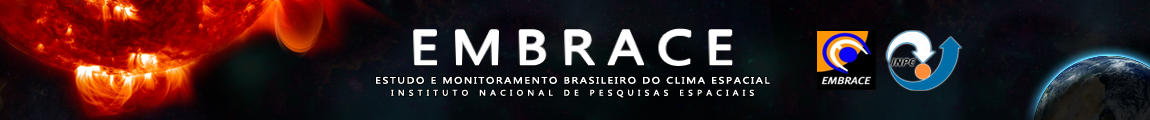
\includegraphics[width=10cm]{embracetopimage.png}}

\title{\Large{\textbf{Briefing Space Weather}}}
\date{2022/05/09}

\begin{document}
\maketitle 

  \thispagestyle{fancy} \section{Sun} 
 \subsection{Responsible: Name}

05/02 – Fast (=$<$ 500 km/s) wind stream; 4 CME c.h.c. toward the Earth; \\ 05/03 – 1 M1, 1 X1 and radio blackout ; Fast (=$<$ 450 km/s) wind stream; 8 CME c.h.c. toward the Earth; \\ 05/04 – 2 M5+ flares, 3 M1 and radio blackout; No fast wind stream; 8 CME c.h.c. toward the Earth; \\ 05/05 – 2 M1 flares; No fast wind stream; 5 CME c.h.c. toward the Earth; \\ 05/06 – No fast wind stream; 5 CME c.h.c. toward the Earth; \\ 05/07 – No fast wind stream; 2 CME c.h.c. toward the Earth; \\ 05/08 – No fast wind stream; 4 CME c.h.c. toward the Earth; \\ 05/09 – No fast wind stream; 1 CME c.h.c. toward the Earth; \\ Prev.: No fast wind up to May 12; for the next 2 days relatively low (30\% M, 5\% X) probability of M / X flares; also, \\ occasionally other CME can present component toward the Earth. \\ c.h.c. – can have a component\section{Sun} 
 \subsection{Responsible: Name}

\begin{itemize} 
 \item WSA-ENLIL (CME 2022-05-03T18:12Z)
\begin{itemize} 
 \item The simulation results indicate that the flank of CME will reach the DSCOVR mission between 2022-05-08T01:00Z and 2022-05-08T15:00Z.
\end{itemize} 
 \item WSA-ENLIL (CME 2022-04-27T08:48Z, 2022-04-27T14:53Z)
\begin{itemize} 
 \item The simulation indicates that the Coronal Mass Ejections’ flanks will reach the DSCOVR mission between 2022-05-11T04:00Z and 2022-05-11T18:00Z. 
\end{itemize} 
 \end{itemize} 
 

    \begin{figure}[H]
        \centering
        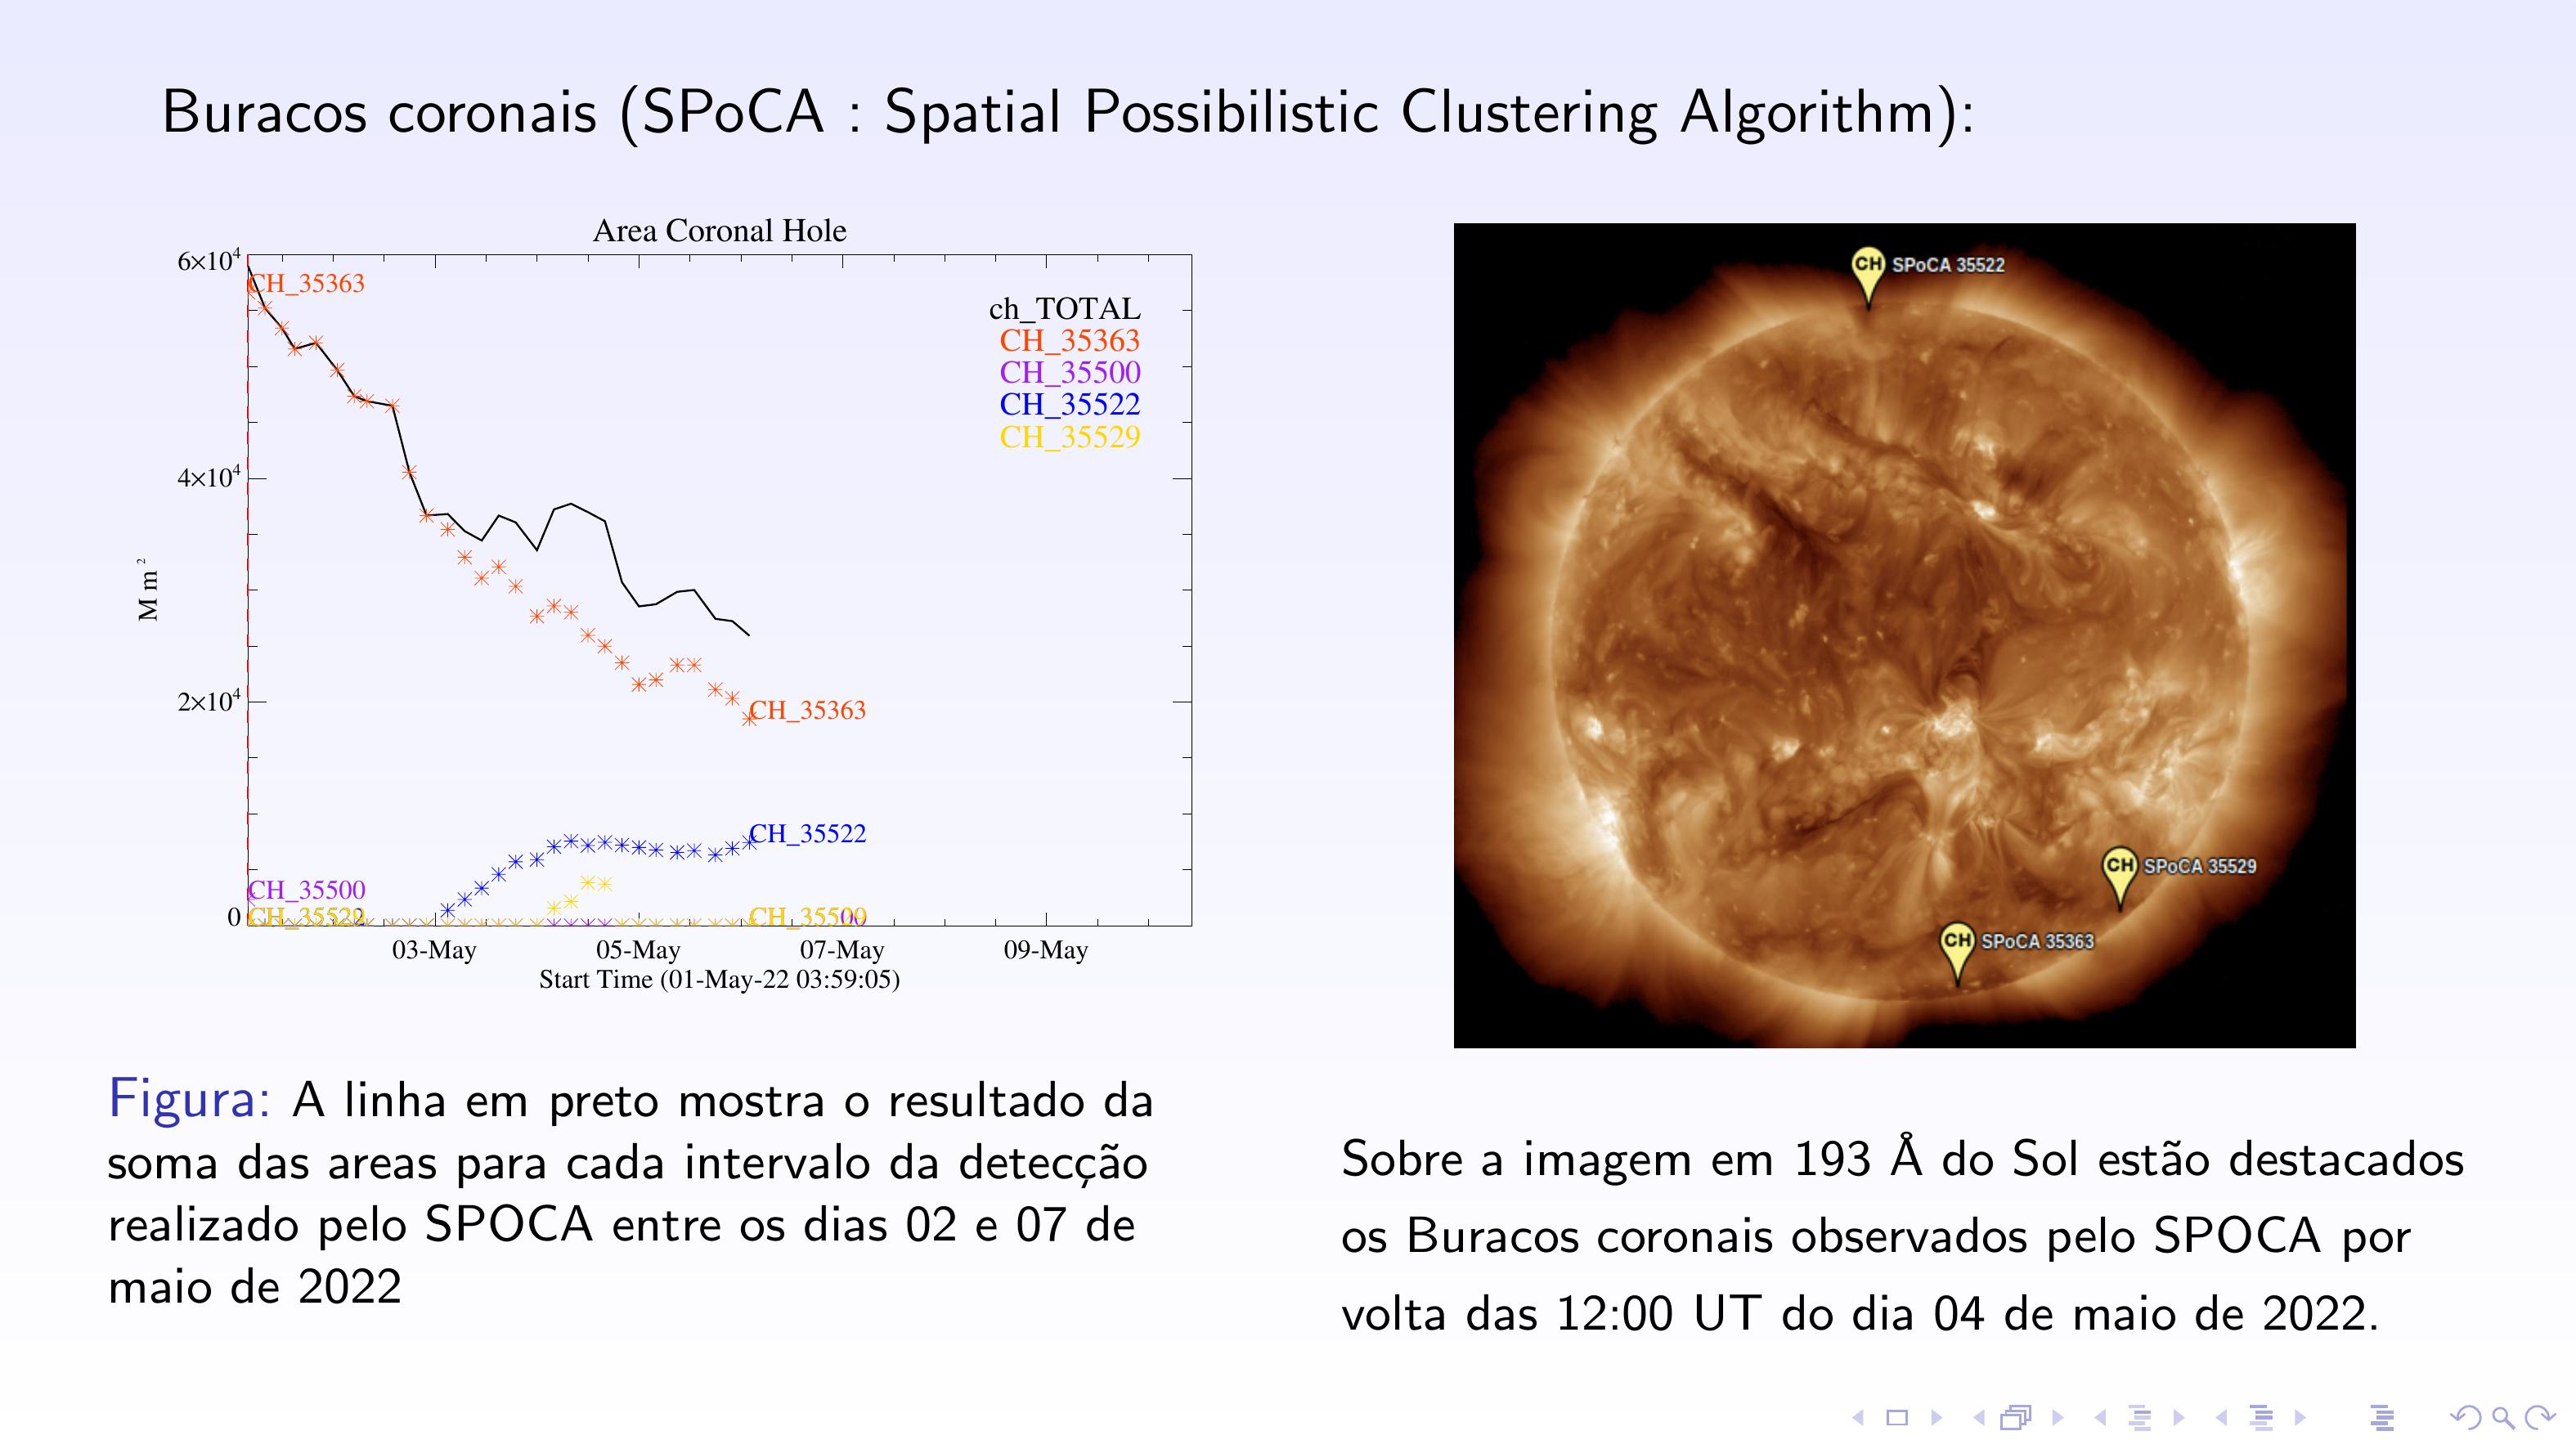
\includegraphics[width=14cm]{./figures/en_outfileSun_0.jpg}
    \end{figure} 
 

    
    \begin{figure}[H]
        \centering
        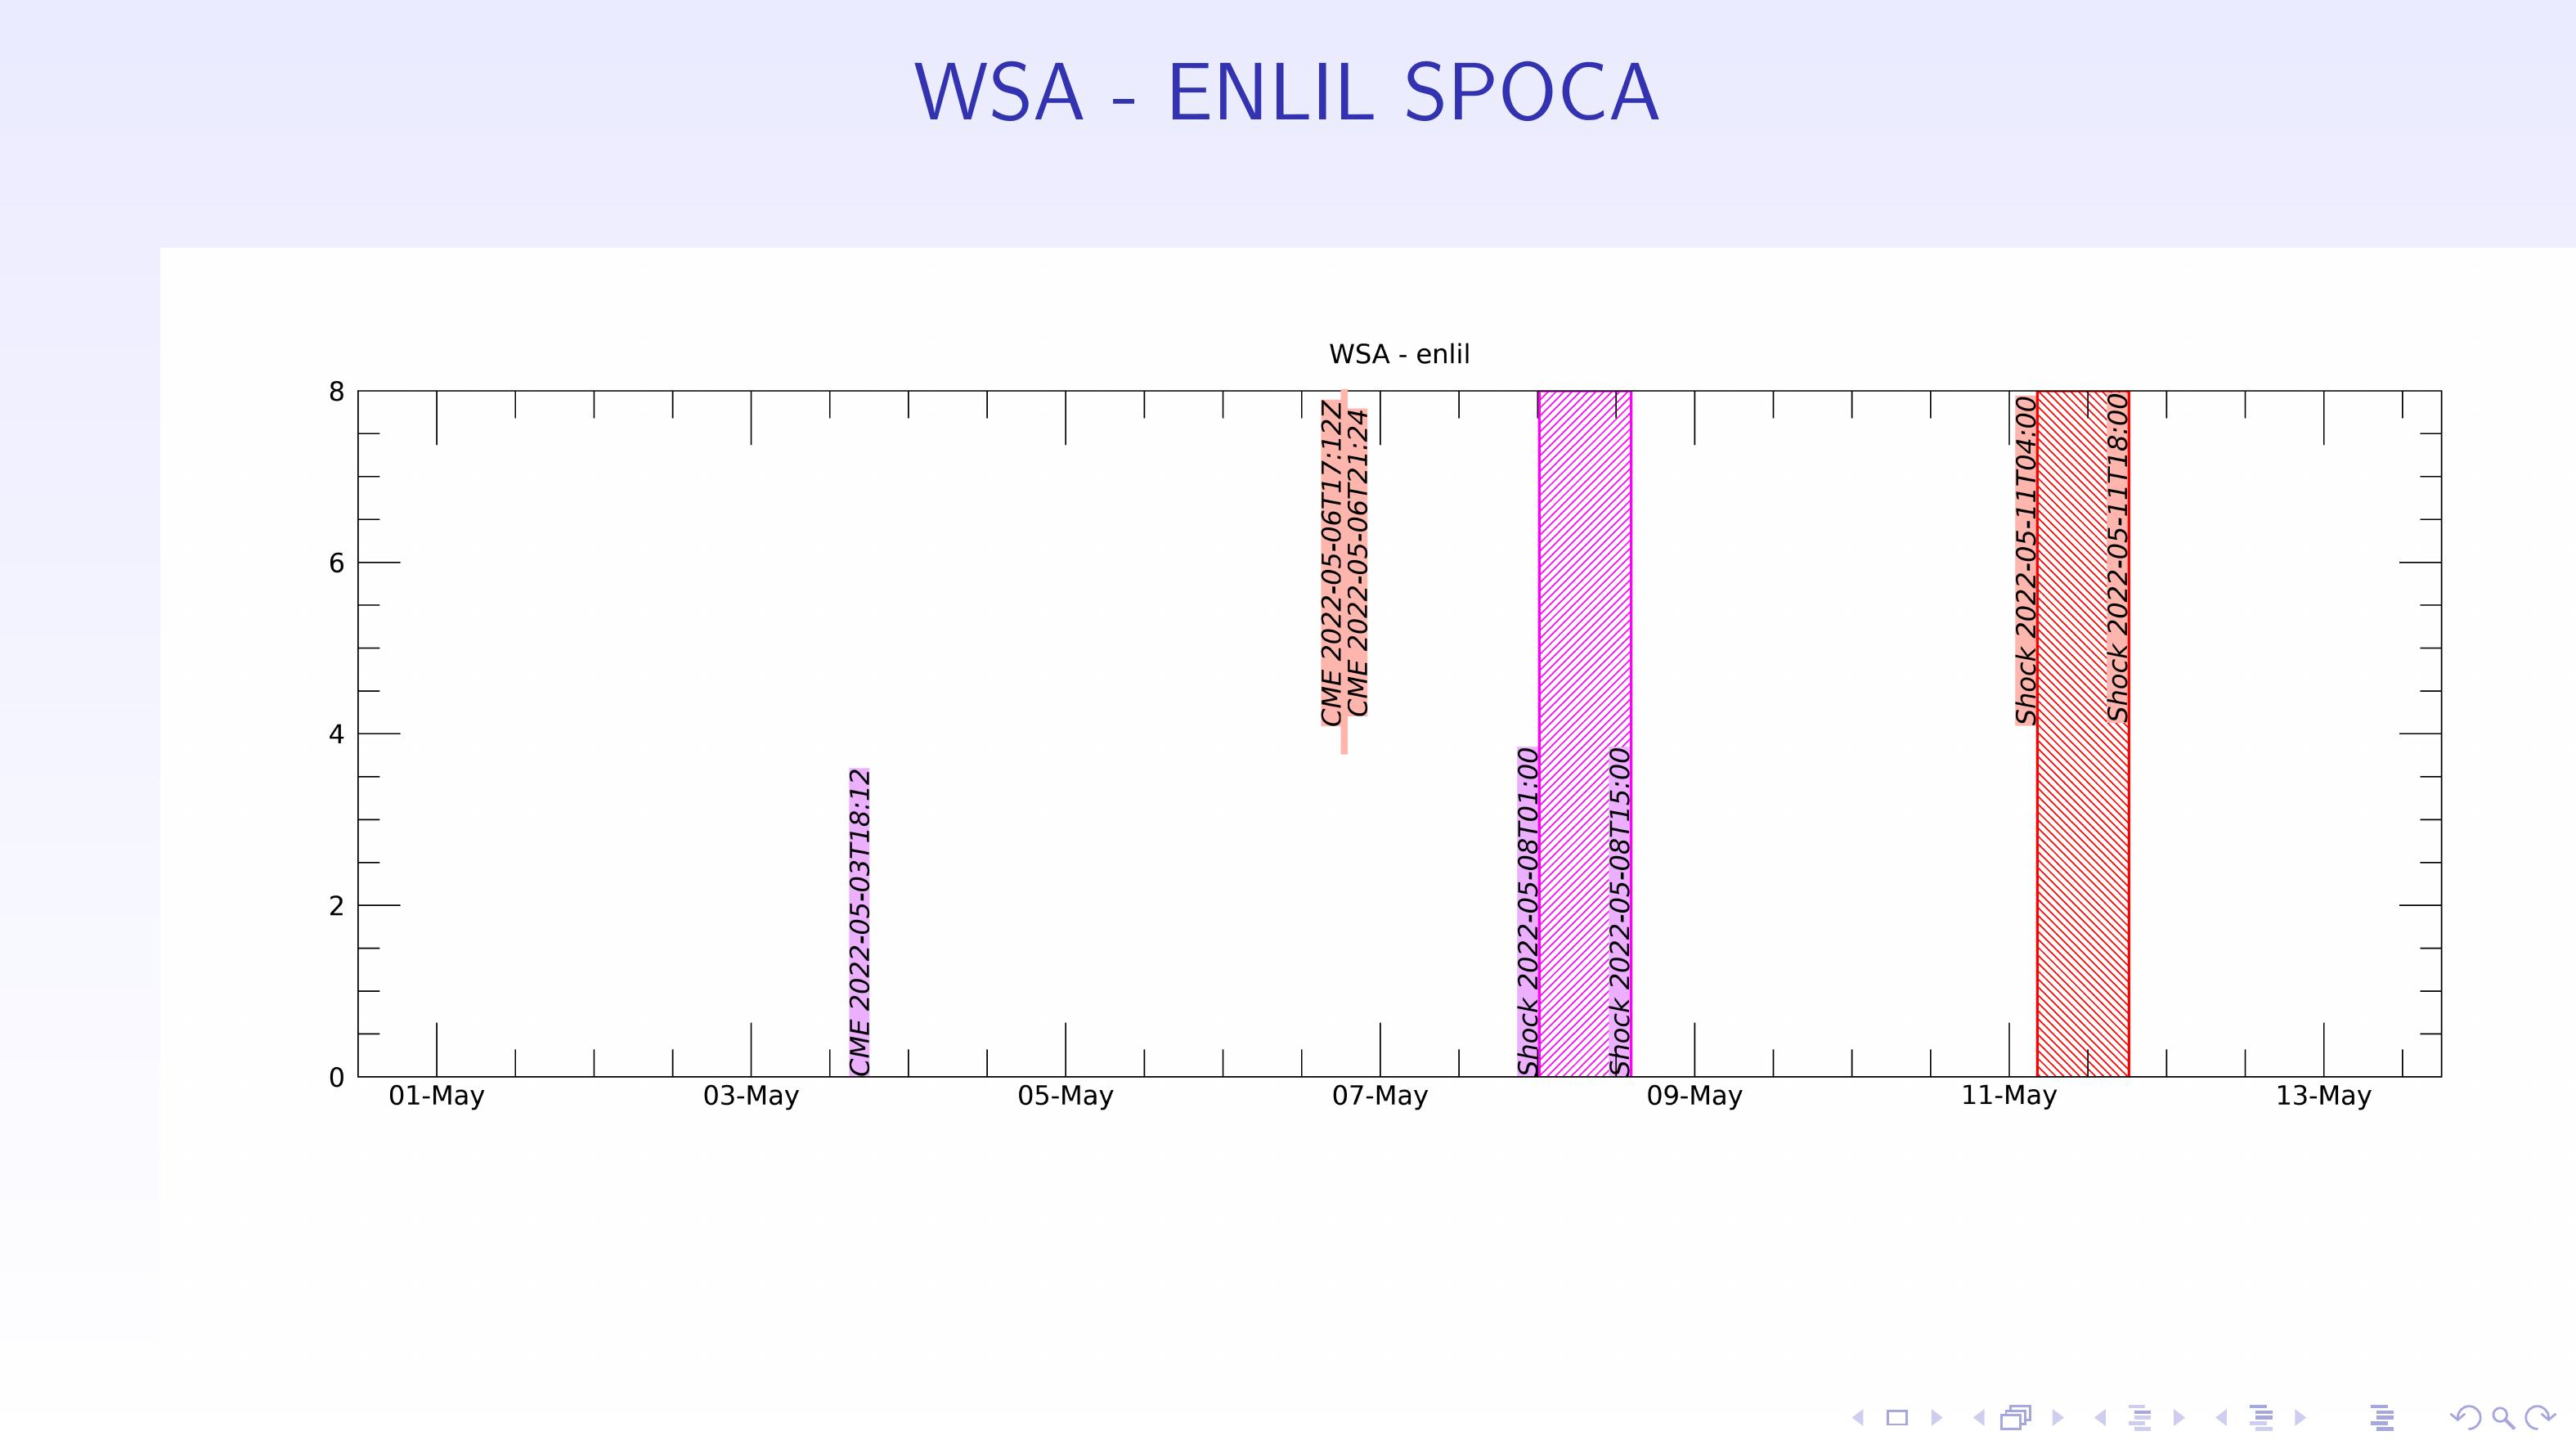
\includegraphics[width=14cm]{./figures/en_outfileSun_1.jpg}
    \end{figure} 
 

    \section{Interplanetary Medium} 
 \subsection{Responsible: Name} 
 
 \begin{figure}[H]
    \centering
    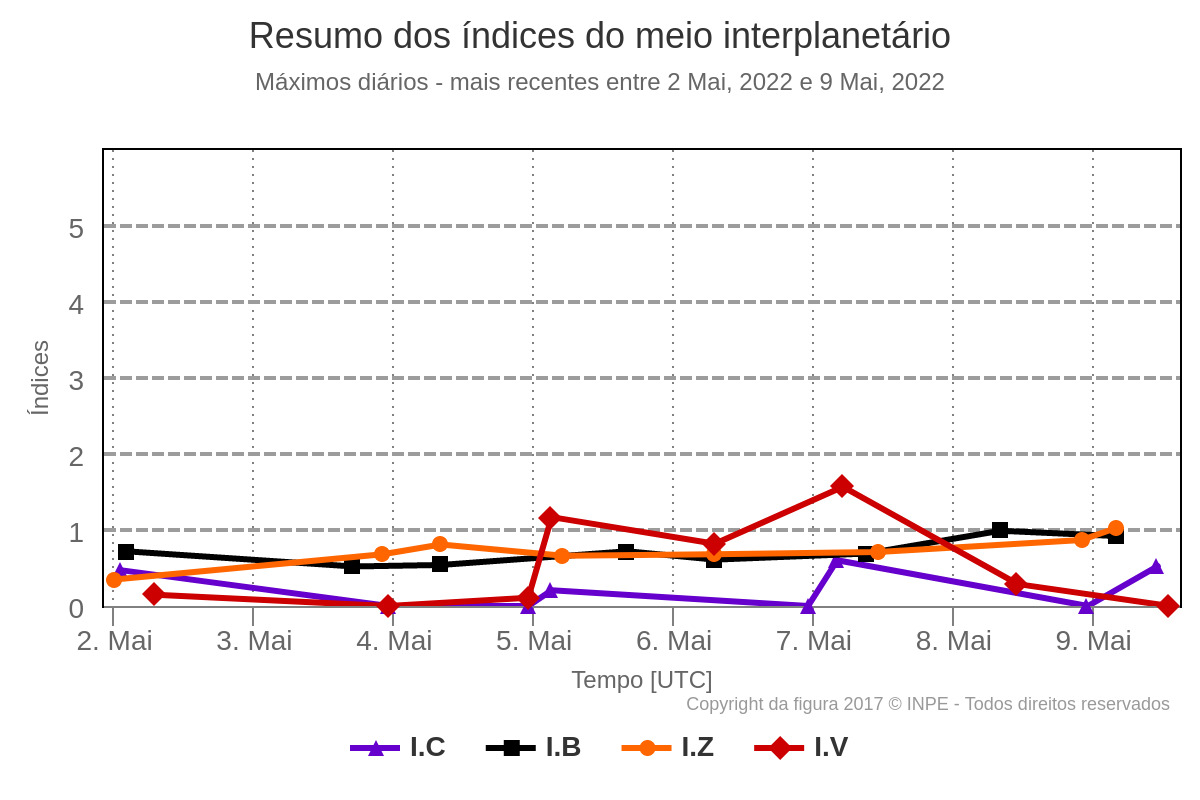
\includegraphics[width=14cm]{./figures//figureMIIndex.png}
\end{figure}
 \begin{itemize}
 \item .
\item The interplanetary medium region in the last week showed a low level of plasma perturbations due to the possible interaction of CME and HSS-like structures identified by the DISCOVERY satellite in the interplanetary medium.
\item  The modulus of the component of the interplanetary magnetic field showed 1 maximum peak : 08/May at 08:30 of ~ 7.9 nT. 
\item The BxBy components showed variations in the analyzed period, both remaining oscillating within the [+5.5, -7.5] nT interval.
\item  The bz field component showed fluctuations with a positive value of 2.61 nT on May 09 at 07:30 and a negative value of -5.11 nT at 04:30 UT on May 09. On average, the Bz component oscillated mostly negative. Conditions favorable to the emergence of geomagnetic disturbances.
\item  The solar wind density oscillated mostly below 5 p/cm³ during the analyzed period with a maximum peak on May 9 at 11:30 am of 16 p/cm³. 
\item The solar wind speed had oscillated mostly below 400 km/s throughout the presenting period. 
\item The magnetopause position was oscillating on average above the typical 10 Re position.
\end{itemize} 
\section{Radiation Belts} 
 \subsection{Responsible: Name} 
 
\begin{figure}[H]
    
                        \centering
   
                             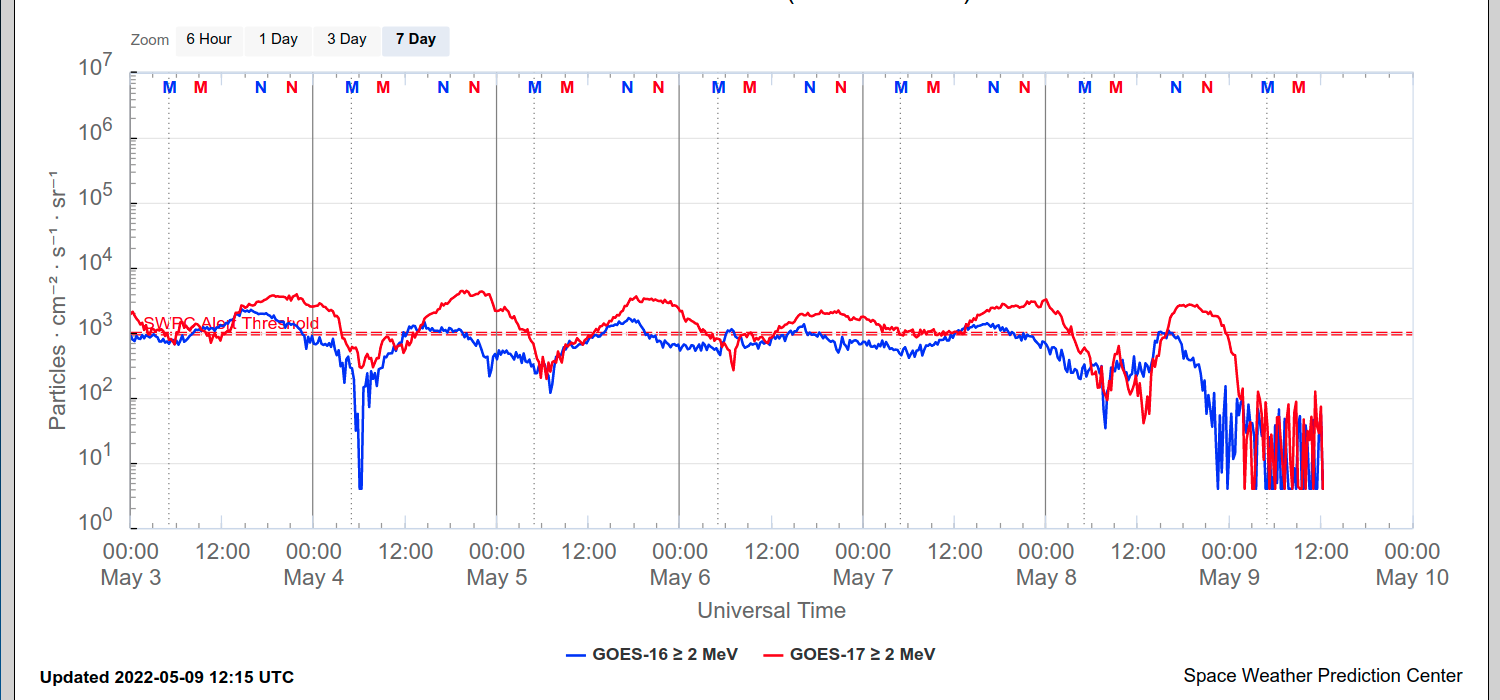
\includegraphics[width=14cm]{./figures//figureRadBelts_0.png}

                             \caption{ High-energy electron flux (> 2MeV) obtained from GOES-16 and GOES-17 satellite. Source}
                        \end{figure}

                     \begin{figure}[H]
    
                        \centering
   
                             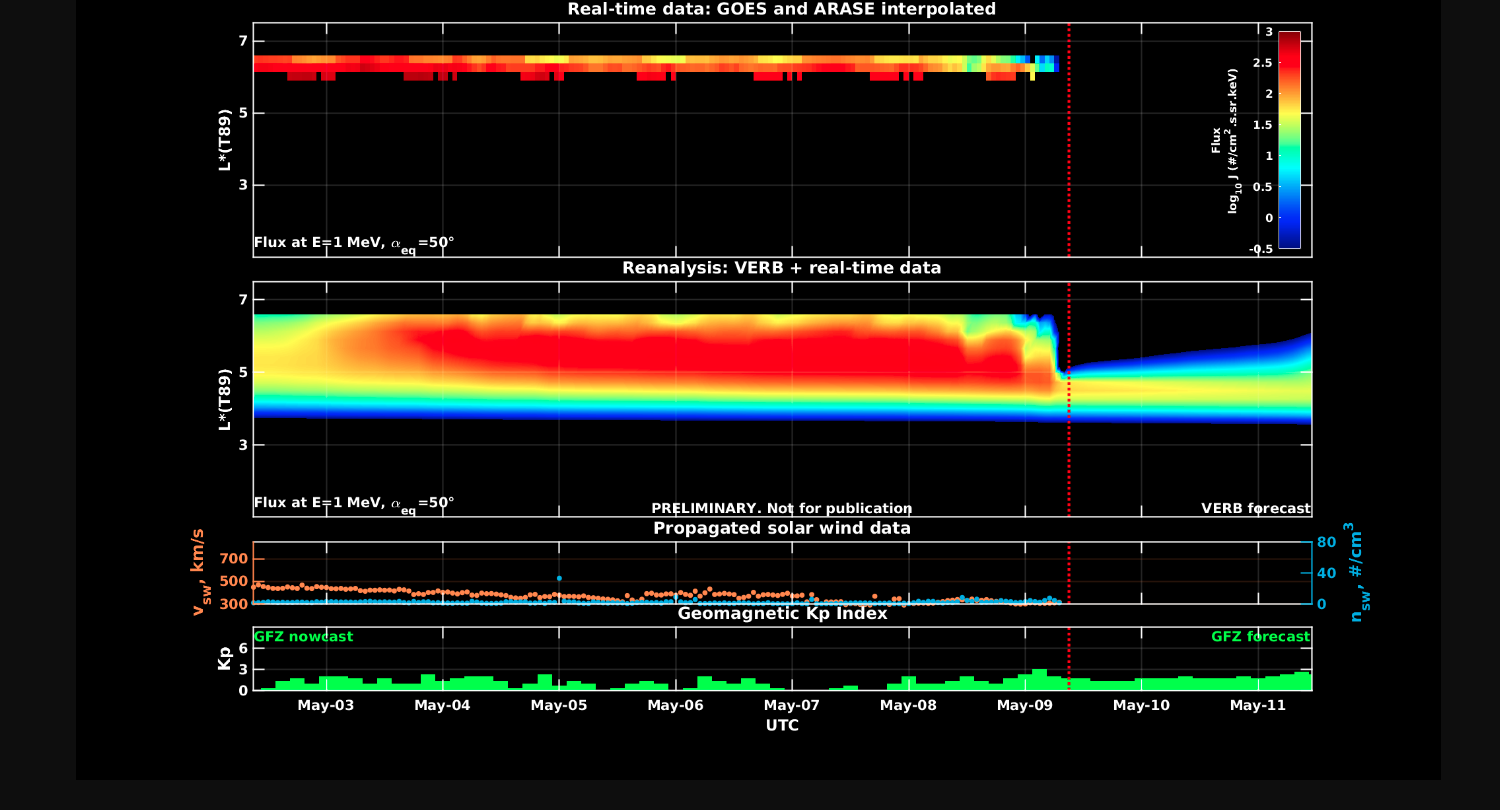
\includegraphics[width=14cm]{./figures//figureRadBelts_1.png}

                             \caption{ high-energy electron flux data (real-time and interpolated) obtained from ARASE, GOES-16, GOES-17 satellites. Reanalysis’s data from VERB code and interpolated electron flux. Solar wind velocity and proton density data from ACE satellite. Source}
                        \end{figure}

                     High-energy electron flux (>2 MeV) in the outer boundary of the outer radiation belt obtained from geostationary satellite data GOES-16 and GOES-17 (Figure 1) is stable around the threshold 103 particles/(cm2 s sr) throughout the week of analysis. Three electron flux decreases were observed on May 4th, 8th, and 9th, respectively. The first decrease is considerably rapid, returning to the threshold of 103 particles/(cm2 s sr). The second decrease reaches approximately 1 order of magnitude and persists for more than 9n hours. The third electron flux decrease reaches approximately 2 orders of magnitude and persists until the last record.    

The GOES-16, GOES-17, and Arase satellite data are analyzed and interpolated to observe the high-energy electron flux variability (1 MeV) in the outer radiation belt (Figure 2). Additionally, the VERB code rebuilds this electron considering the Ultra Low Frequency (ULF) waves' radial diffusion. The simulation (VERB code) shows that the first electron flux decrease occurs only at the outer boundary of the outer radiation belt, the second reaches L-shell = 6.0, and the third reaches L-shell – 5.0. These electron flux variability occurred concomitantly with the arrival of solar wind structures and ULF wave activities. However, it is important to point out that the data from the ARASE satellite are not available for the week under analysis to confirm the L-shell level of these electron flux variabilities.\section{ULF Waves} 
 \subsection{Responsible: Name} 
 
\begin{figure}[H]
    
                        \centering
   
                             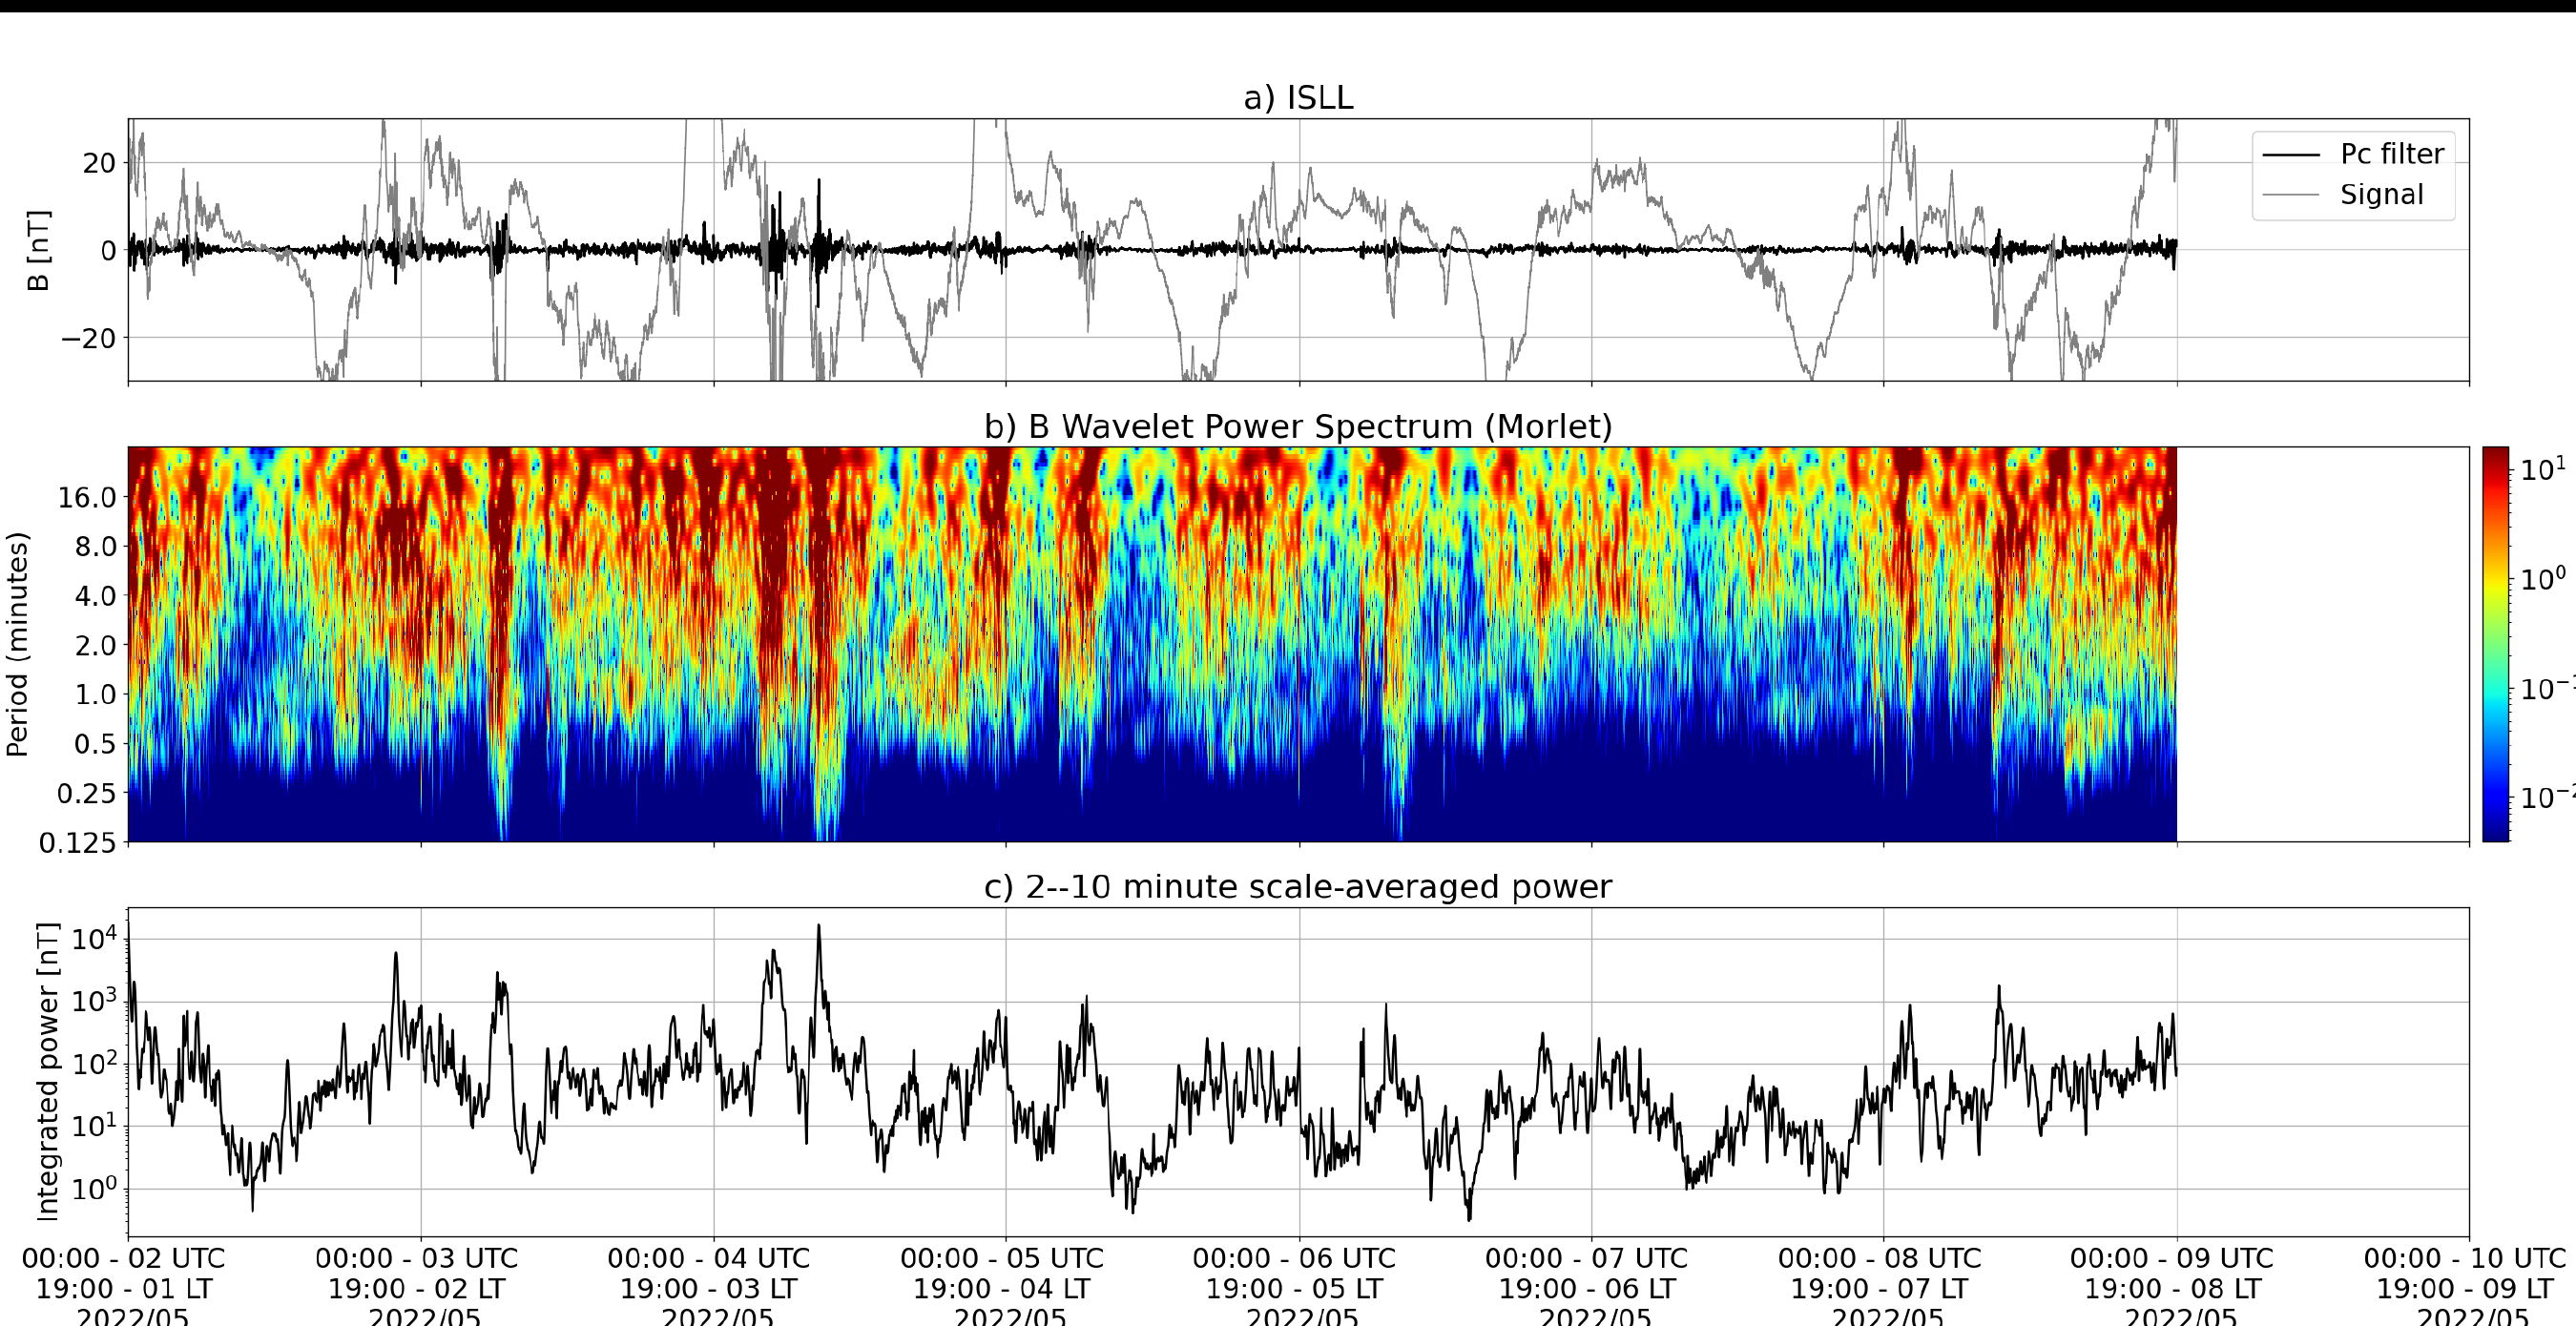
\includegraphics[width=14cm]{./figures//figureULF_0.png}

                             \caption{a) signal of the total magnetic 
                              field measured in the ISLL Station of the CARISMA 
                              network in gray, together with the fluctuation in the 
                              range of Pc5 in black. b) Wavelet power spectrum of the 
                              filtered signal. c) Average spectral power in the ranges 
                              from 2 to 10 minutes (ULF waves).}
                        \end{figure}

                     \begin{figure}[H]
    
                        \centering
   
                             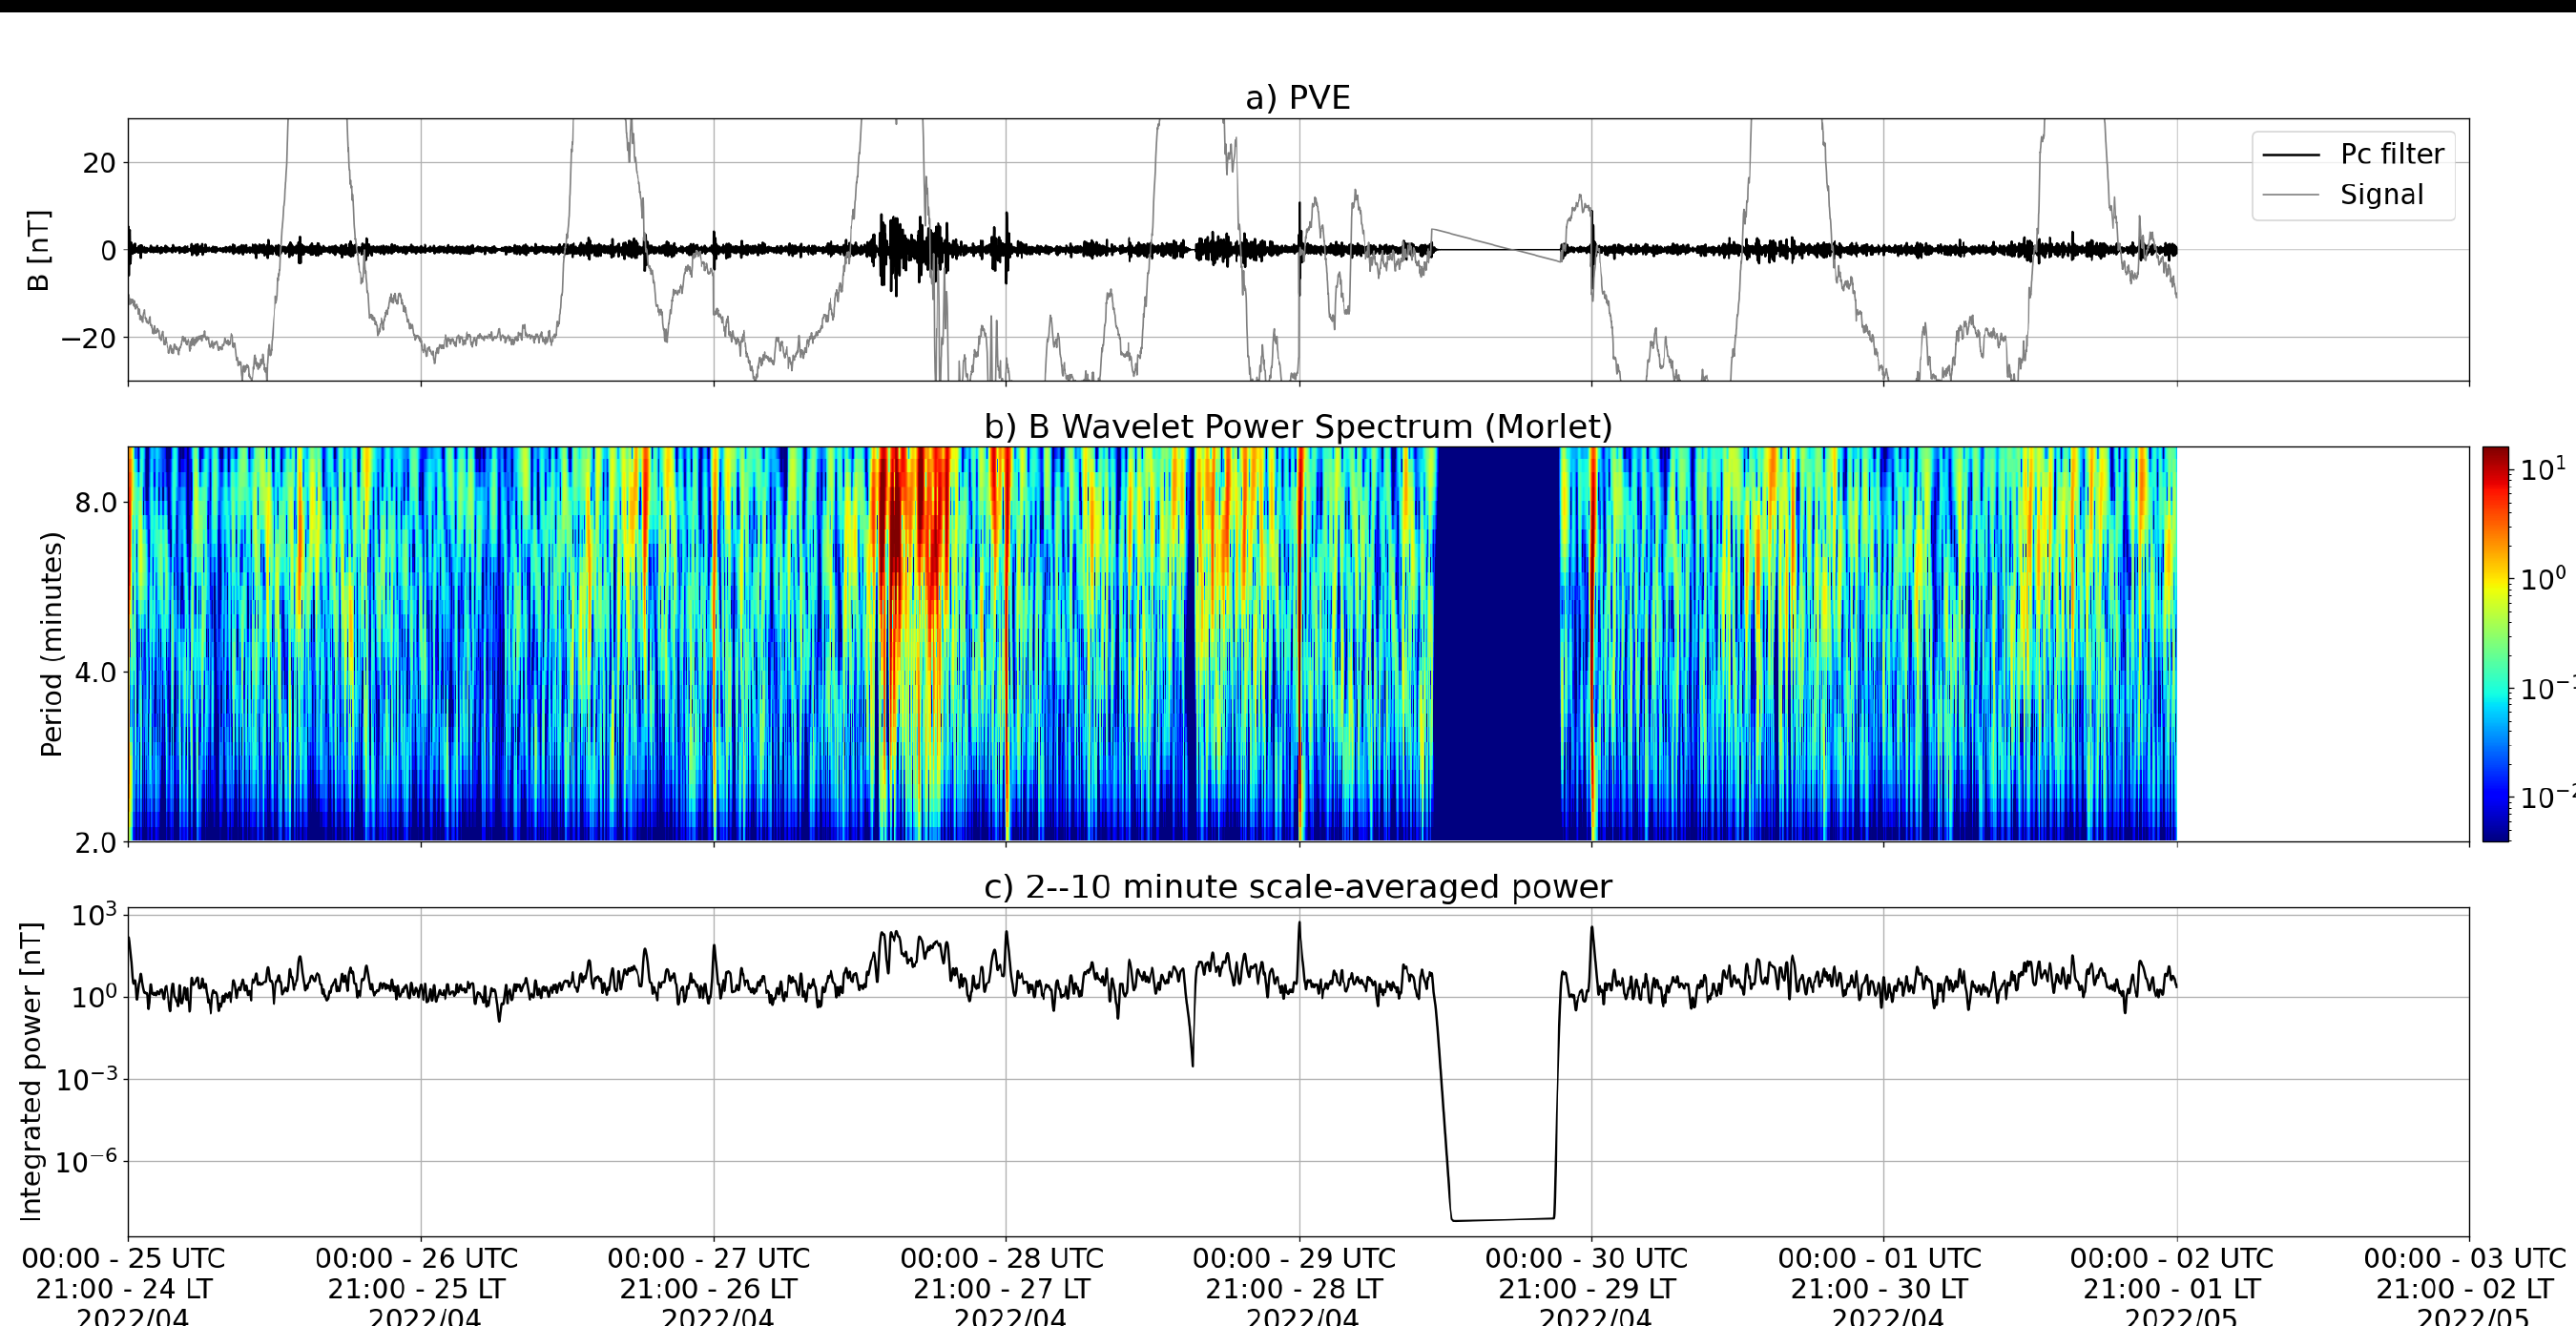
\includegraphics[width=14cm]{./figures//figureULF_1.png}

                             \caption{a) signal of the total magnetic field 
                              measured in the EMBRACE network in gray, together with
                               the fluctuation in the range of Pc5 in black. b)
                                Wavelet power spectrum of the filtered signal. c) 
                                Average spectral power in the ranges from 2 to 10
                                 minutes (ULF waves).}
                        \end{figure}

                     \begin{figure}[H]
    
                        \centering
   
                             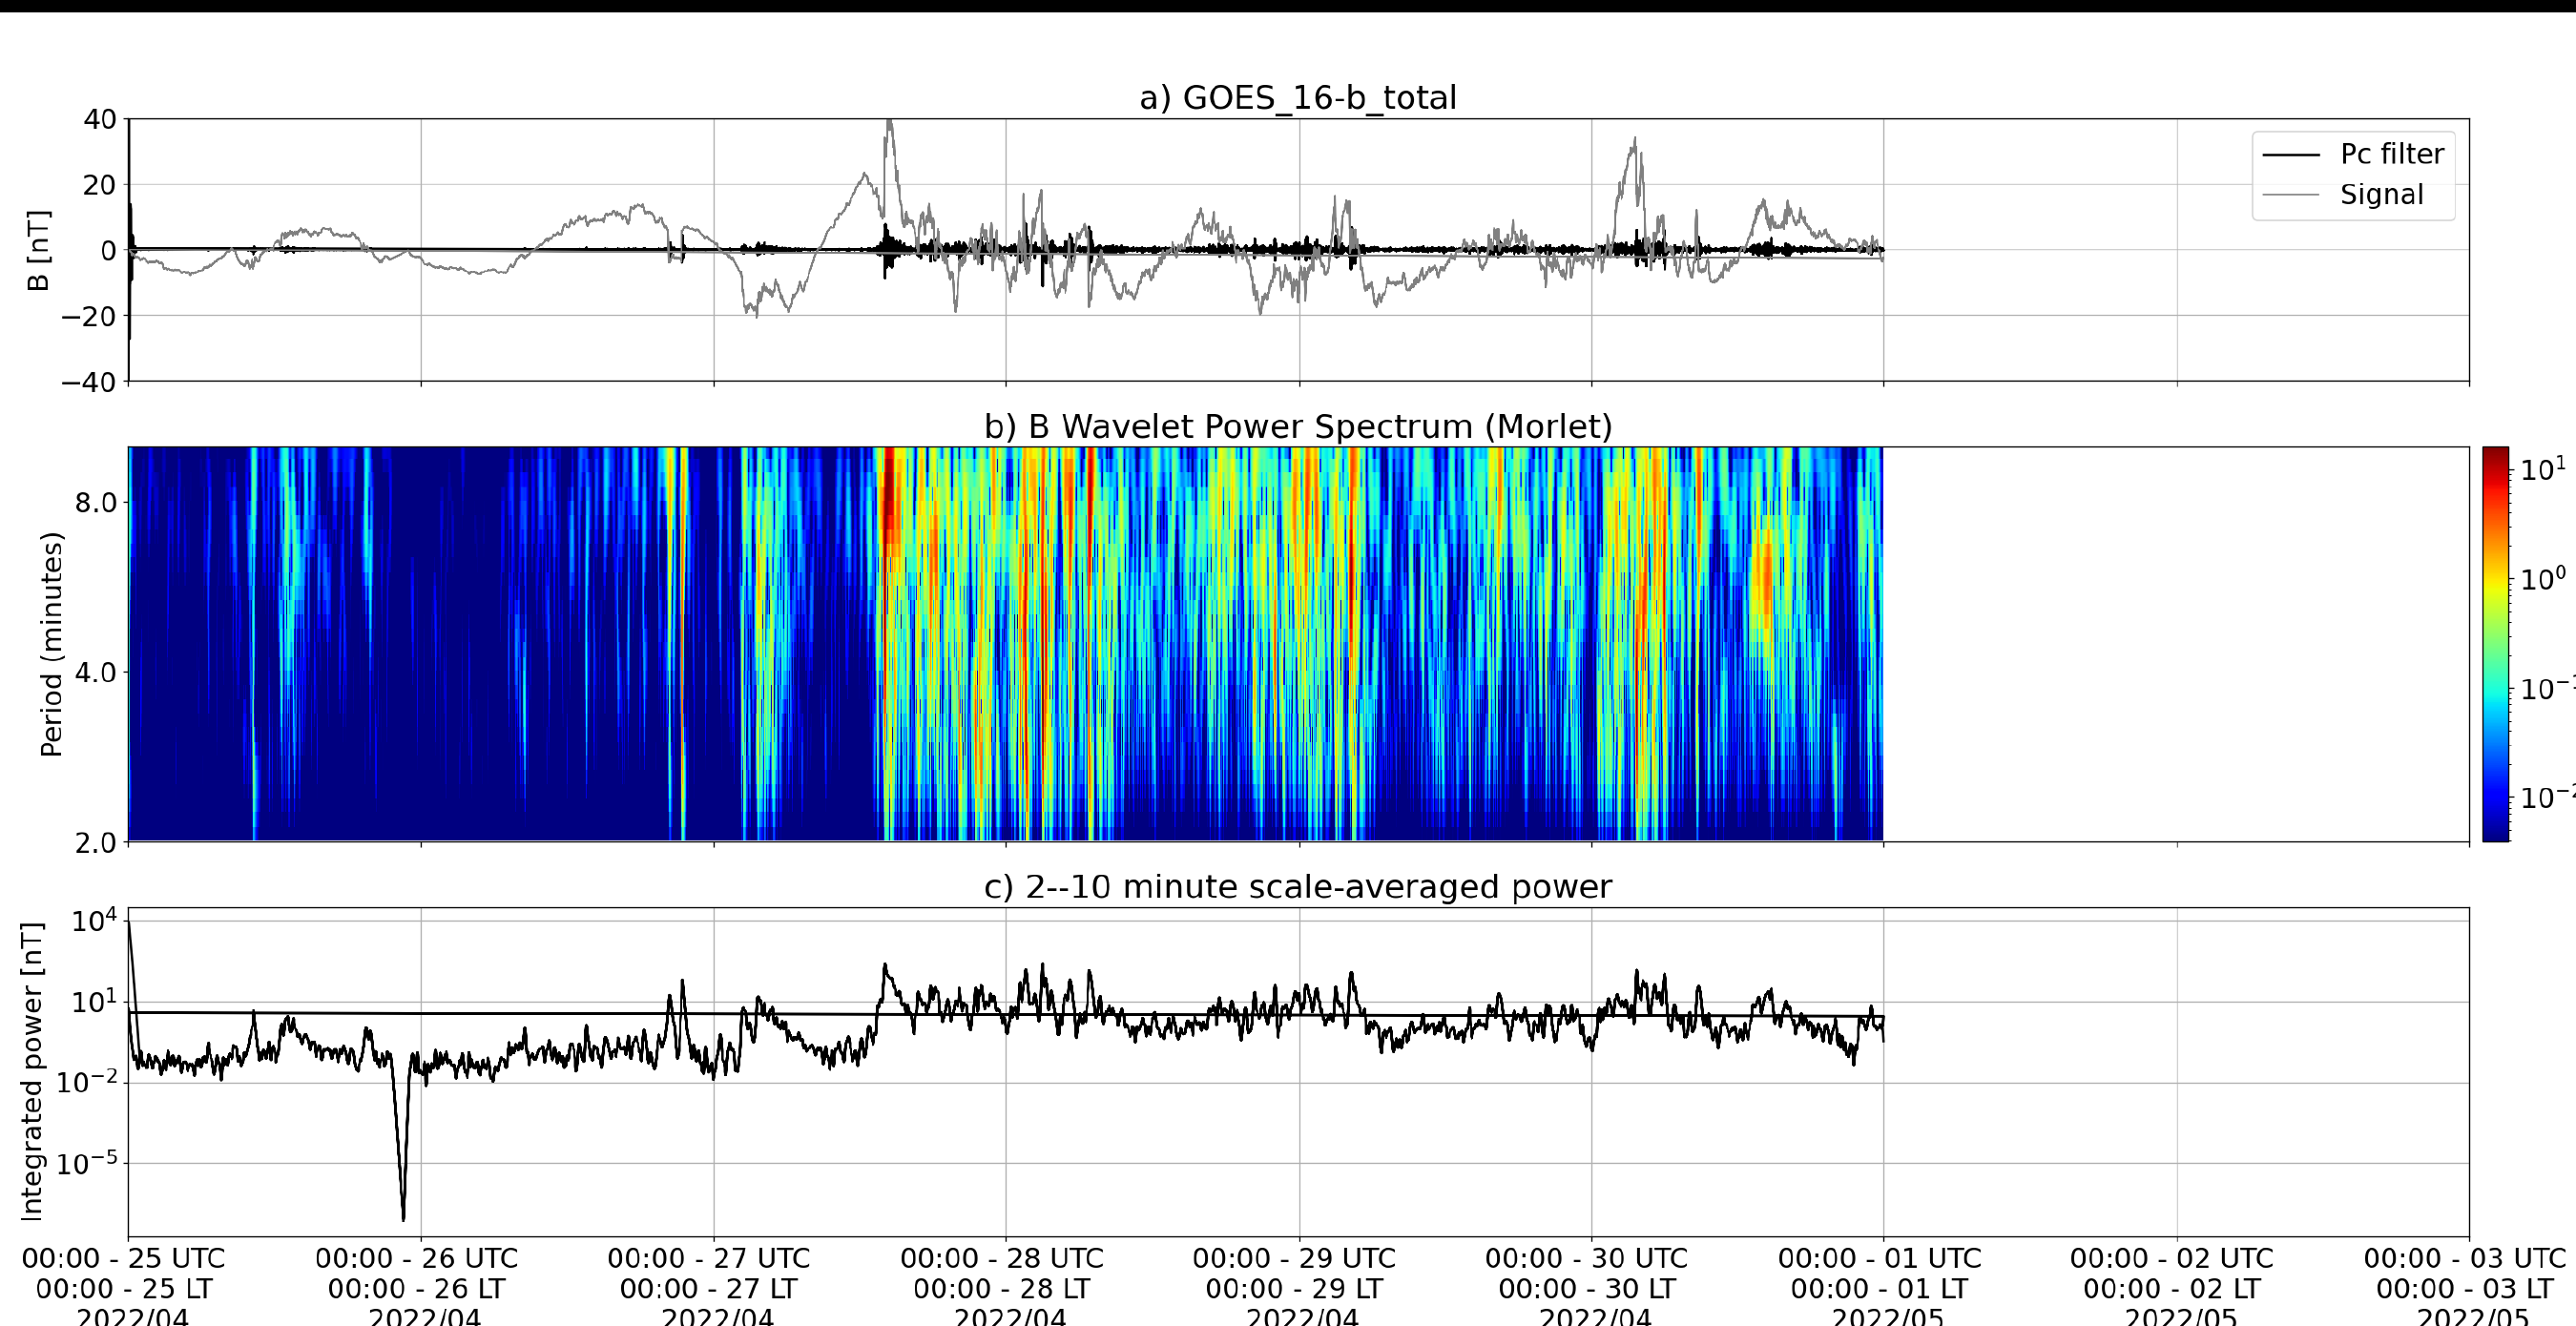
\includegraphics[width=14cm]{./figures//figureULF_2.png}

                             \caption{a) signal of the total magnetic field 
                              measured by the GOES 16 satellite, together with the 
                              fluctuation in the range of Pc5 in black. b) Wavelet 
                              power spectrum of the filtered signal. c) Average 
                              spectral power in the ranges from 2 to 10 minutes 
                              (ULF waves).}
                        \end{figure}

                     The ULF wave activity shows an increase in power from the 3rd of May in
the form of irregular and short-duration pulsations, detected from high
latitudes to the magnetometers at low latitudes of the EMBRACE network
(Figure 2, SMS), the same activity repeats on May 4th. The activity continues
until the 7th of May with reduced power. On day 8, there is a further
increase in spectral power, now with continuous characteristics, mainly at
high latitudes. This period is possibly under the effect of a corrotant
interaction region (CIR) and also periods with an increase in the density of
the solar wind and component of the magnetic field of the solar wind
predominantly in the south direction.
Summary
10/10
The ULF wave activity shows an increase in power from the 3rd of May in the form of irregular and short-duration pulsations, detected from high latitudes to the magnetometers at low latitudes of the EMBRACE network (Figure 2, SMS), the same activity repeats on May 4th. The activity continues until the 7th of May with reduced power. On day 8, there is a further increase in spectral power, now with continuous characteristics, mainly at high latitudes. This period is possibly under the effect of a corrotant interaction region (CIR) and also periods with an increase in the density of the solar wind and component of the magnetic field of the solar wind predominantly in the south direction.\section{Ondas EMIC} 
 \subsection{Responsável: Name} 
 
\begin{figure}[H]
    
                        \centering
   
                             \includegraphics[width=14cm]{./figures//figureEMIC_1.png}

                        \end{figure}

                     \section{Geomagnetism} 
 \subsection{Responsible: Name} 
 
\begin{figure}[H]
    
                        \centering
   
                             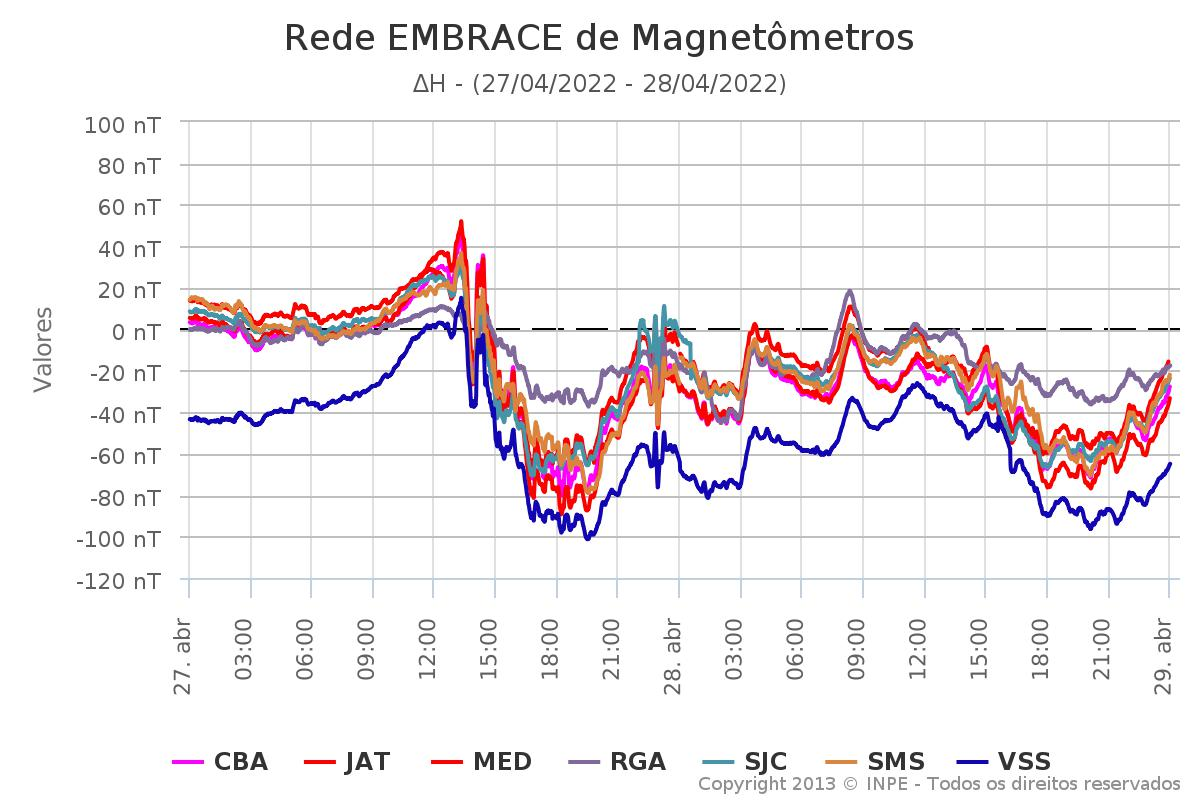
\includegraphics[width=14cm]{./figures//figureGeomag_0.png}

                        \end{figure}

                     \begin{figure}[H]
    
                        \centering
   
                             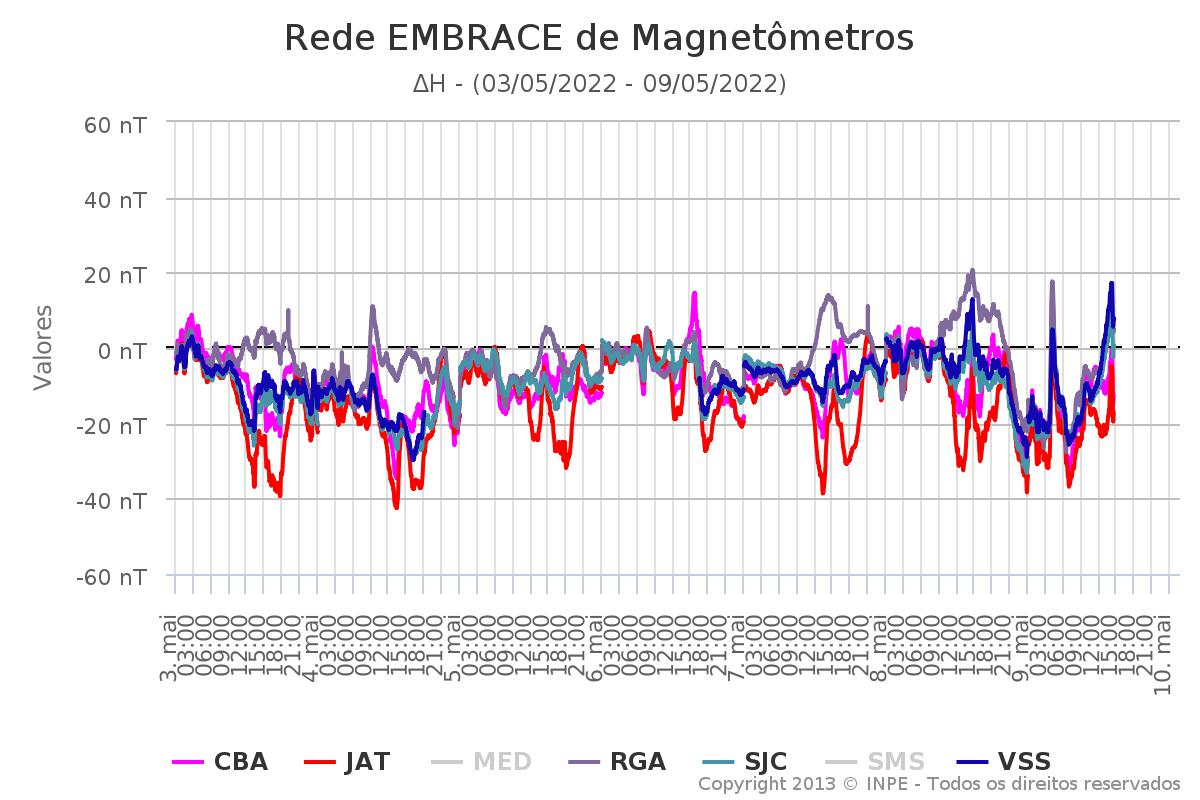
\includegraphics[width=14cm]{./figures//figureGeomag_1.png}

                        \end{figure}

                     \begin{figure}[H]
    
                        \centering
   
                             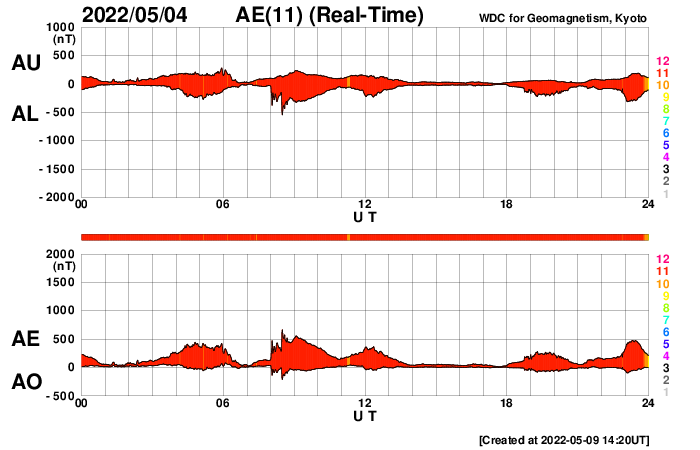
\includegraphics[width=14cm]{./figures//figureGeomag_2.png}

                        \end{figure}

                     \begin{figure}[H]
    
                        \centering
   
                             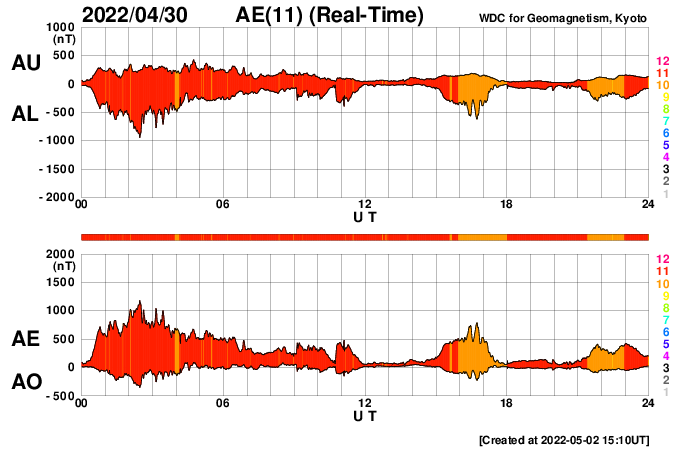
\includegraphics[width=14cm]{./figures//figureGeomag_3.png}

                        \end{figure}

                     \begin{figure}[H]
    
                        \centering
   
                             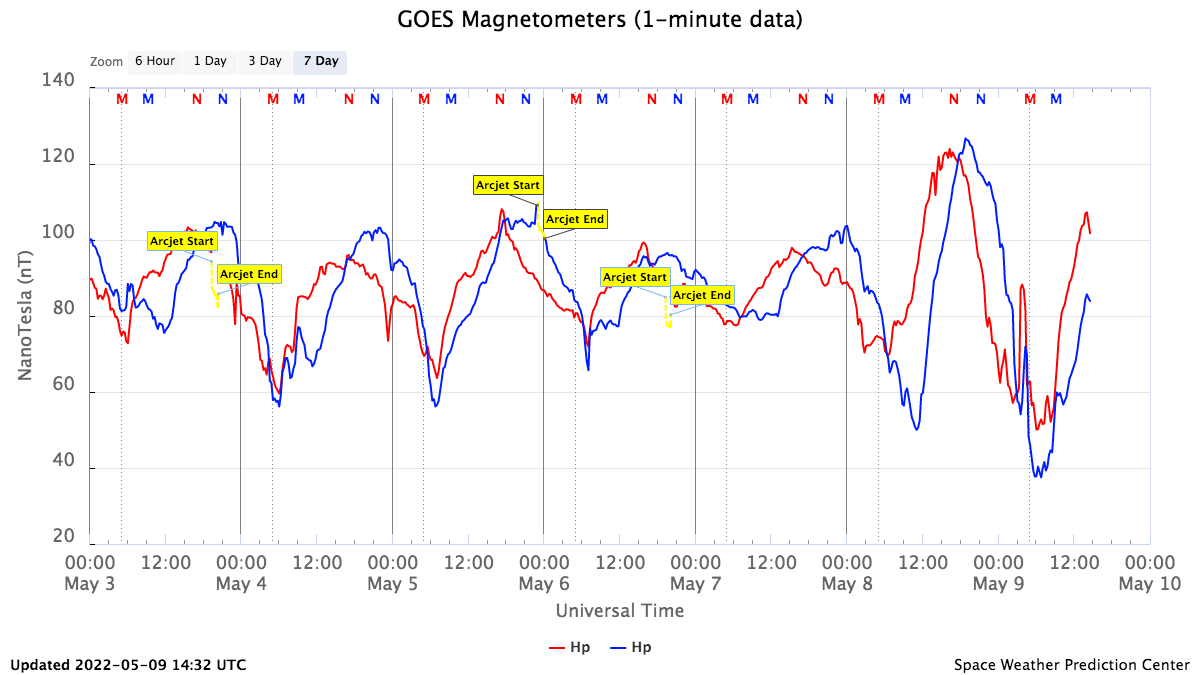
\includegraphics[width=14cm]{./figures//figureGeomag_4.png}

                        \end{figure}

                     \begin{figure}[H]
    
                        \centering
   
                             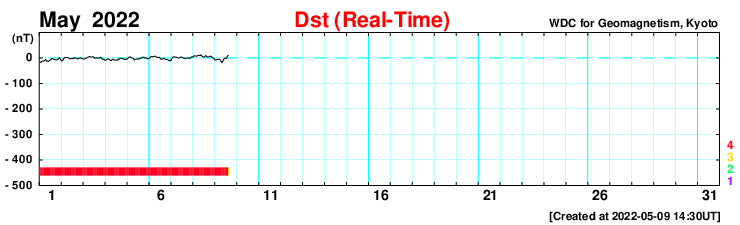
\includegraphics[width=14cm]{./figures//figureGeomag_5.png}

                        \end{figure}

                     \begin{figure}[H]
    
                        \centering
   
                             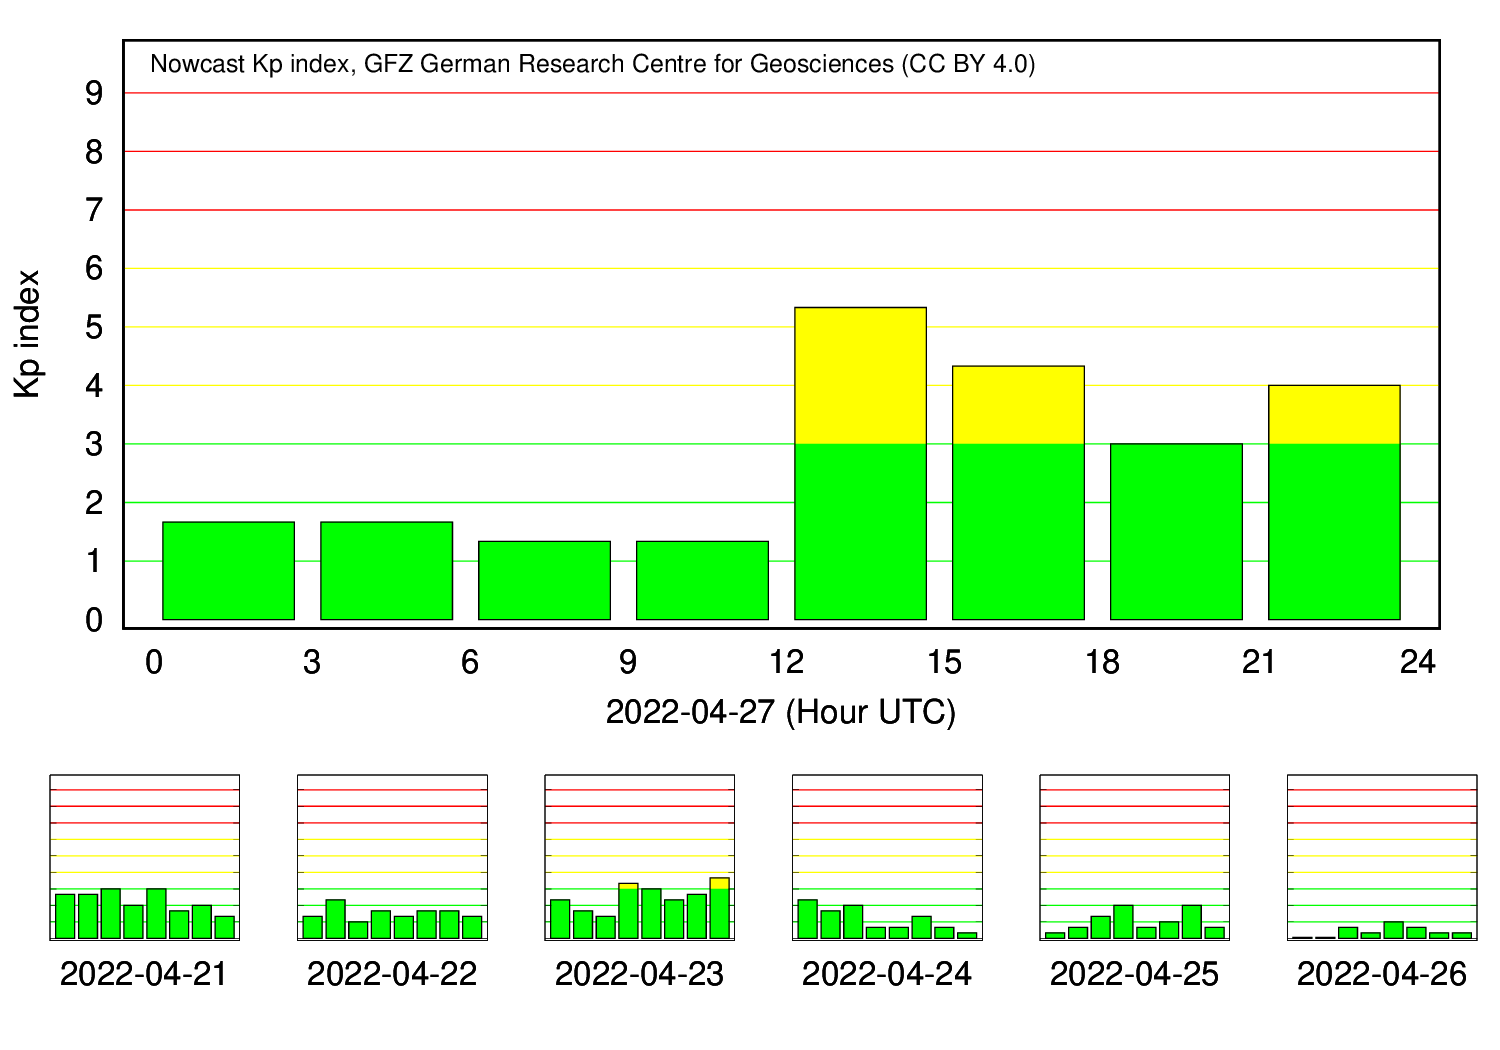
\includegraphics[width=14cm]{./figures//figureGeomag_6.png}

                        \end{figure}

                     \begin{itemize} 
\begin{itemize} 
 \item - Data from the Embrace magnetometer network showed instabilities throughout the period, with some events highlighted:
 \end{itemize} 
\item The highest H instabilities were registered on May 3, 8 and 9
\begin{itemize} 
 \item - Geomagnetic activity was unsettled, with the Dst index reaching around zero. The highest Kp of the week was 3o.
 \end{itemize} 
\begin{itemize} 
 \item - The auroral activity was intensified on May 4 and 9.
 \end{itemize} 
\begin{itemize} 
 \item - Magnetic field measured in the orbit of the GOES satellite showed disturbances on May 09.
 \end{itemize} 
\end{itemize} 
\section{Ionosphere} 
 \subsection{Responsible: Name} 
 
\textbf{Boa Vista: }

 \begin{itemize}
\item There were spread F during all days in this week.
\item The Es layers reached scale 4 on day 07. 
\end{itemize}
\begin{figure}[H]
    \centering
    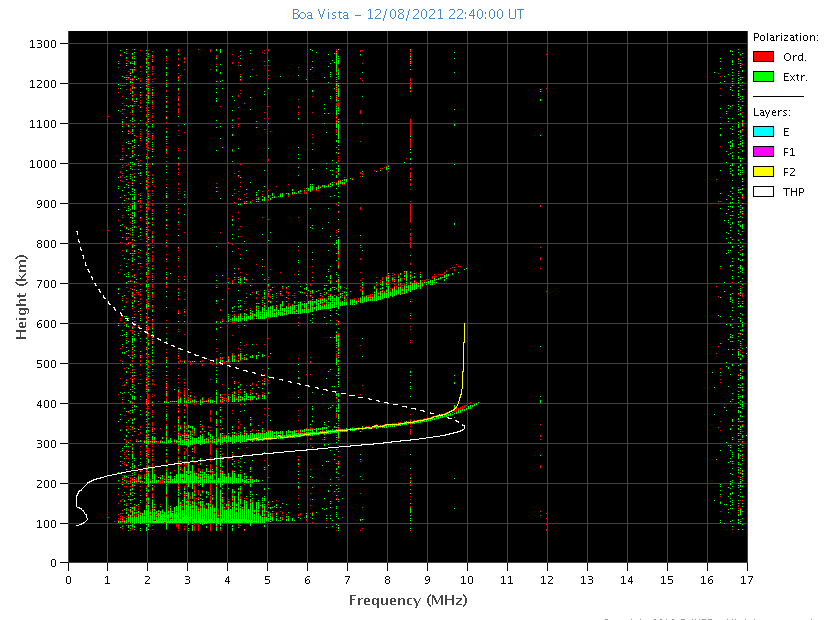
\includegraphics[width=14cm]{./figures//BoaVista.png}
\end{figure}

\textbf{Cachoeira Paulista:}

 \begin{itemize}
\item There were not spread F in this week.
\item The Es layers reached scale 2 during this all week. 
\end{itemize}
\begin{figure}[H]
    \centering
    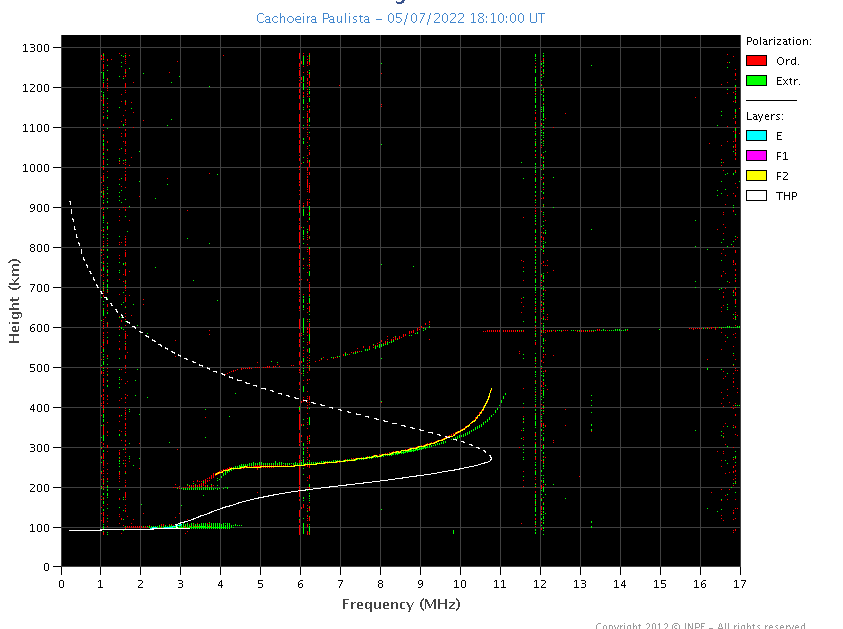
\includegraphics[width=14cm]{./figures//CachoeiraPaulista.png}
\end{figure}

\textbf{São Luís: }

 \begin{itemize}
\item There were spread F during all days in this week.
\item The Es layers reached scale 5 on day 05. 
\end{itemize}
\begin{figure}[H]
    \centering
    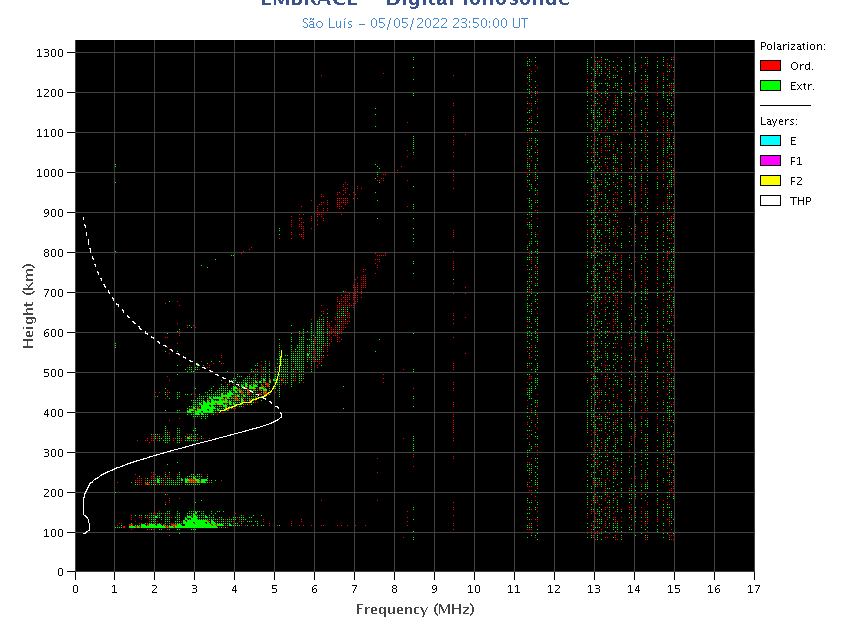
\includegraphics[width=14cm]{./figures//SãoLuís.png}
\end{figure}

\section{SCintilation} 
 \subsection{Responsible: Name} 
 
In this report on the S4 scintillation index, data from FRTZ in Fortaleza/CE, STSN 
in Sinop/MG, UFBA in Bahía/BA and SJCE in São José dos Campos/SP are 
presented. The S4 index tracks the presence of irregularities in the ionosphere 
having a spatial scale ~ 360 m. 
The stations STSN, STNT and SJCE did not present relevant values of the S4 
index throughout the week. In the FRTZ station, a case appeared with S4 values 
above 0.4. The most important was recorded in the morning of 04/25 (Figure 1, 
upper panel). In the lower panel of Figure 1, the affected satellites located to the 
northwest of the FRTZ appear. Ionograms at the same time and location show 
the typical spread in the main trace. This fact together with the position of 
satellites with S4 values > 0.15 shown in the Figure 1 indicate the presence of an 
irregularity in the ionospheric plasma due to a typical plasma bubble at this time 
and at these latitudes close to the geomagnetic equator. 

    \begin{figure}[H]
        \centering
        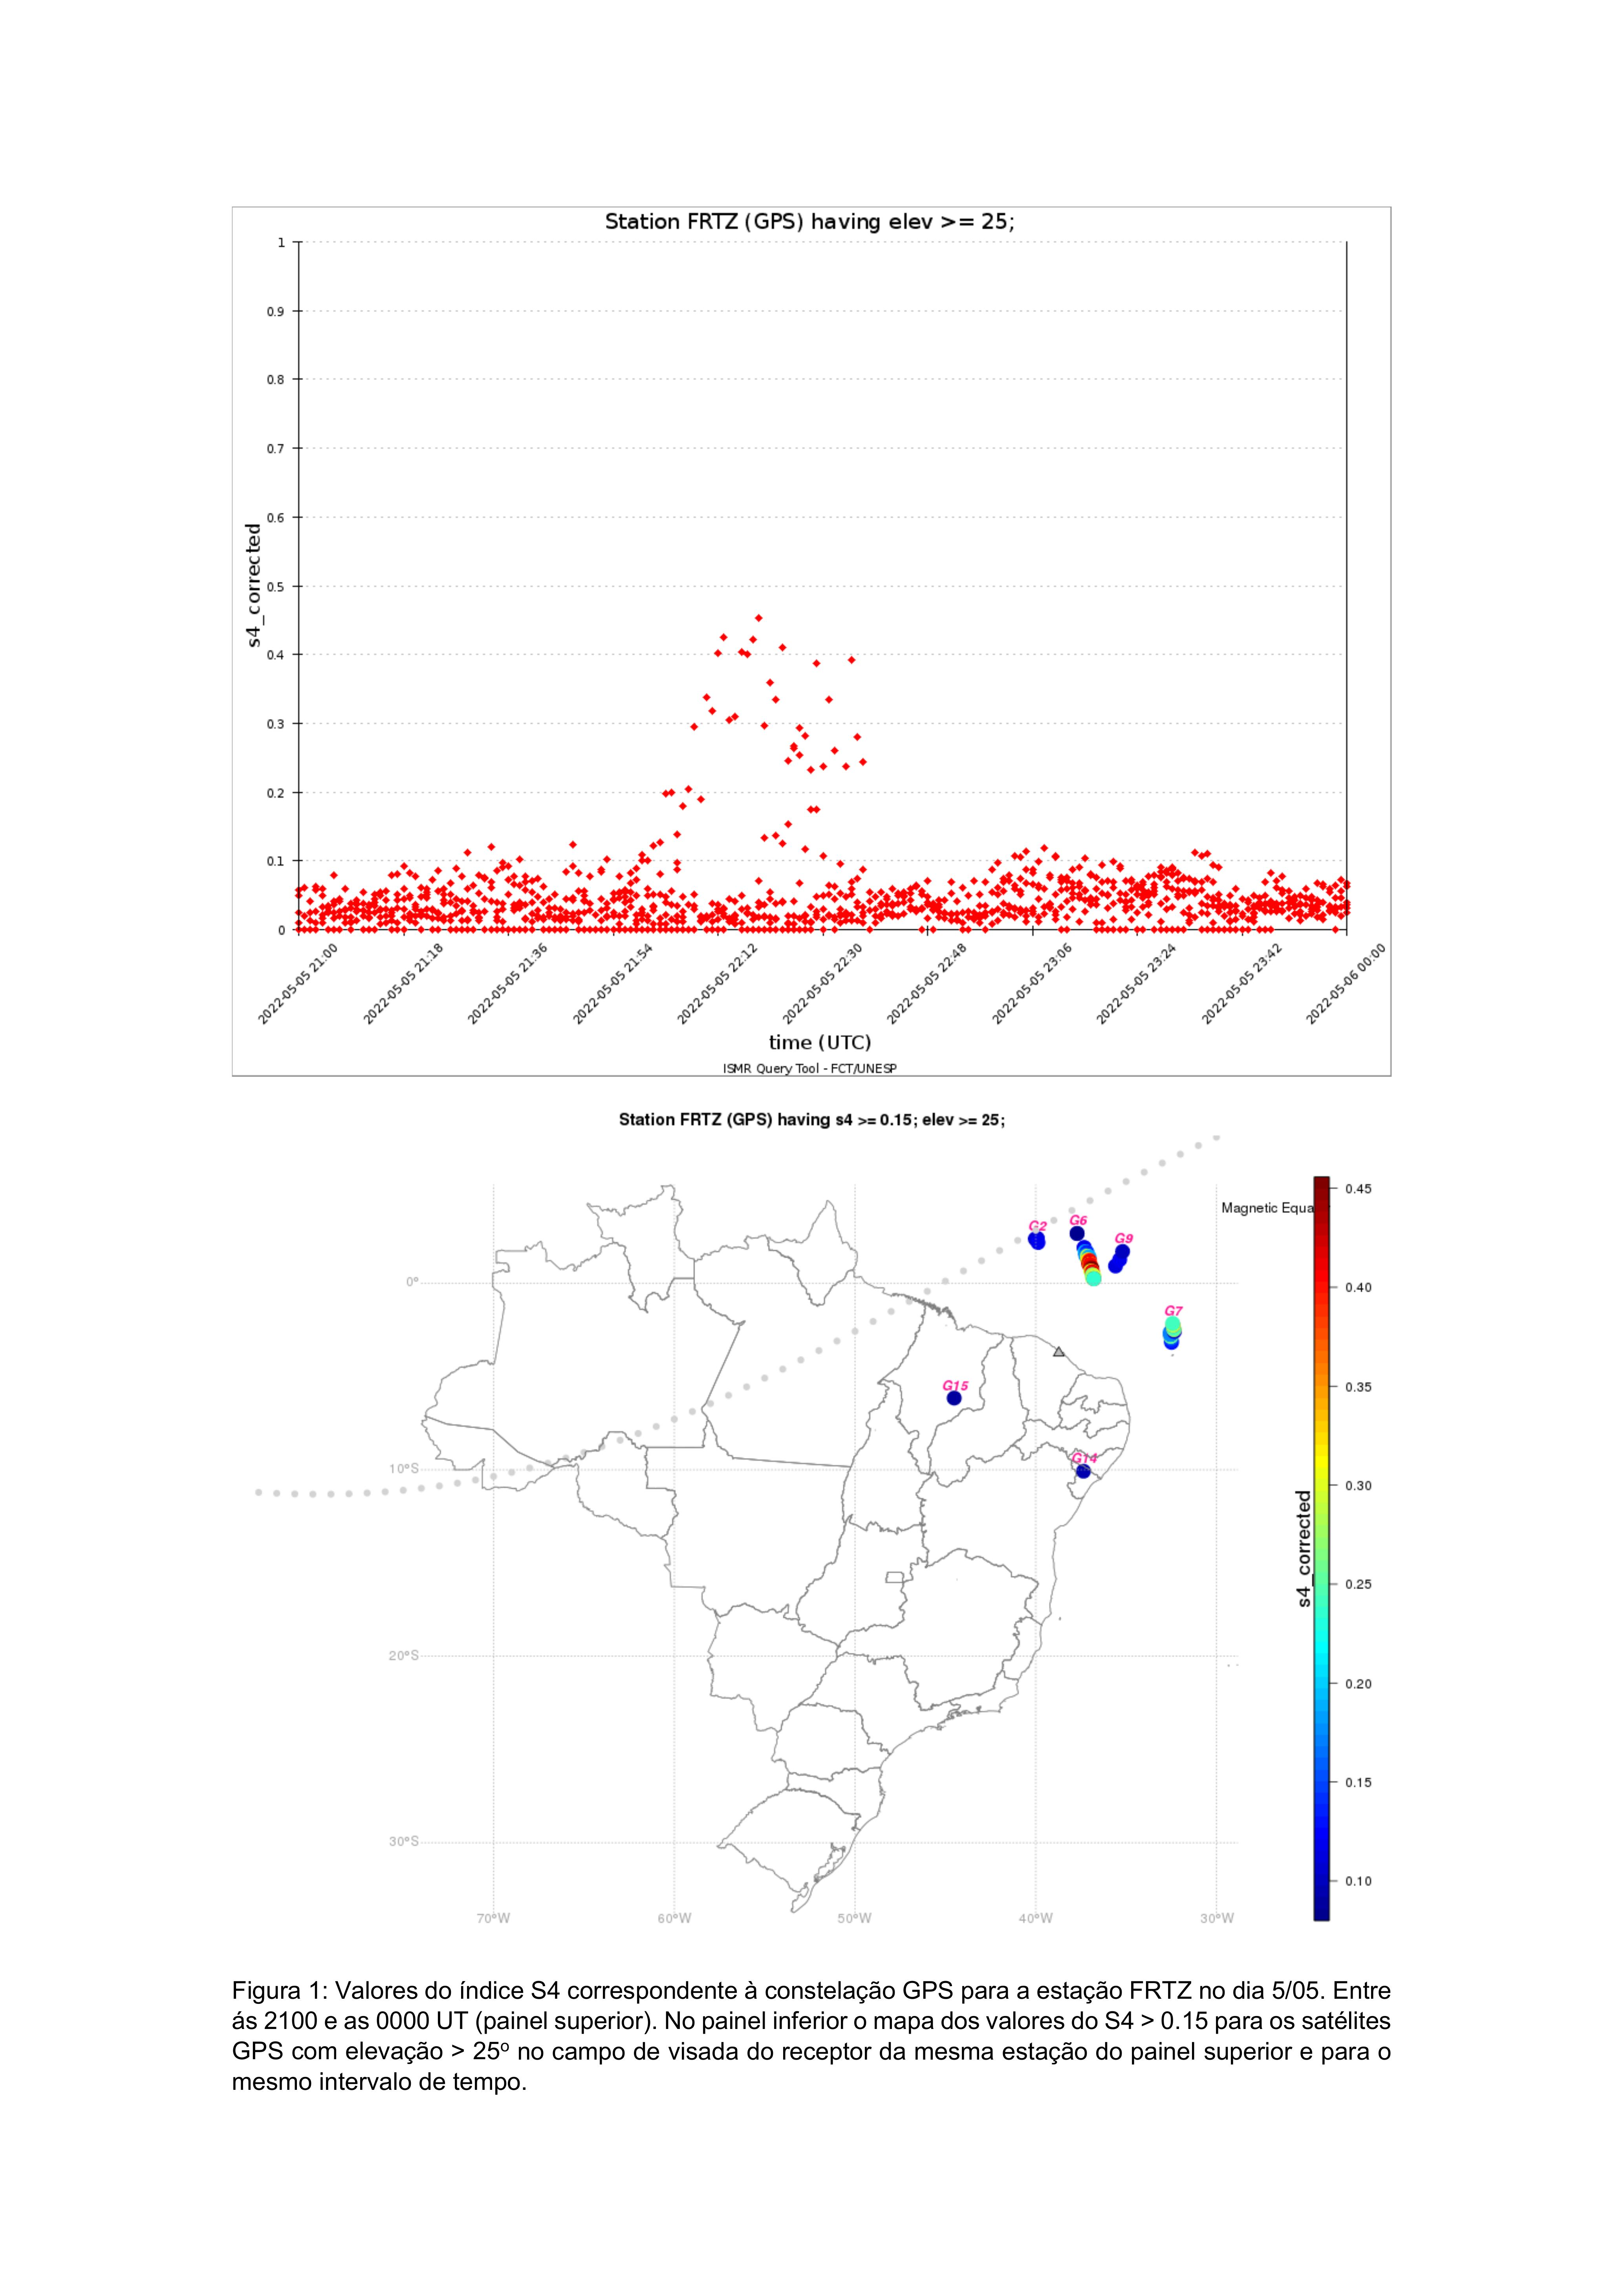
\includegraphics[width=14cm]{./figures/en_outfileScint_0.jpg}
    \end{figure} 
 

    
    \begin{figure}[H]
        \centering
        
\includegraphics[width=14cm]{./figures/en_outfileScint_1.jpg}
    \end{figure} 
 

    \section{All-Sky Imager} 
 \subsection{Responsible: Name} 
 
\begin{figure}[H]
    
                        \centering
   
                             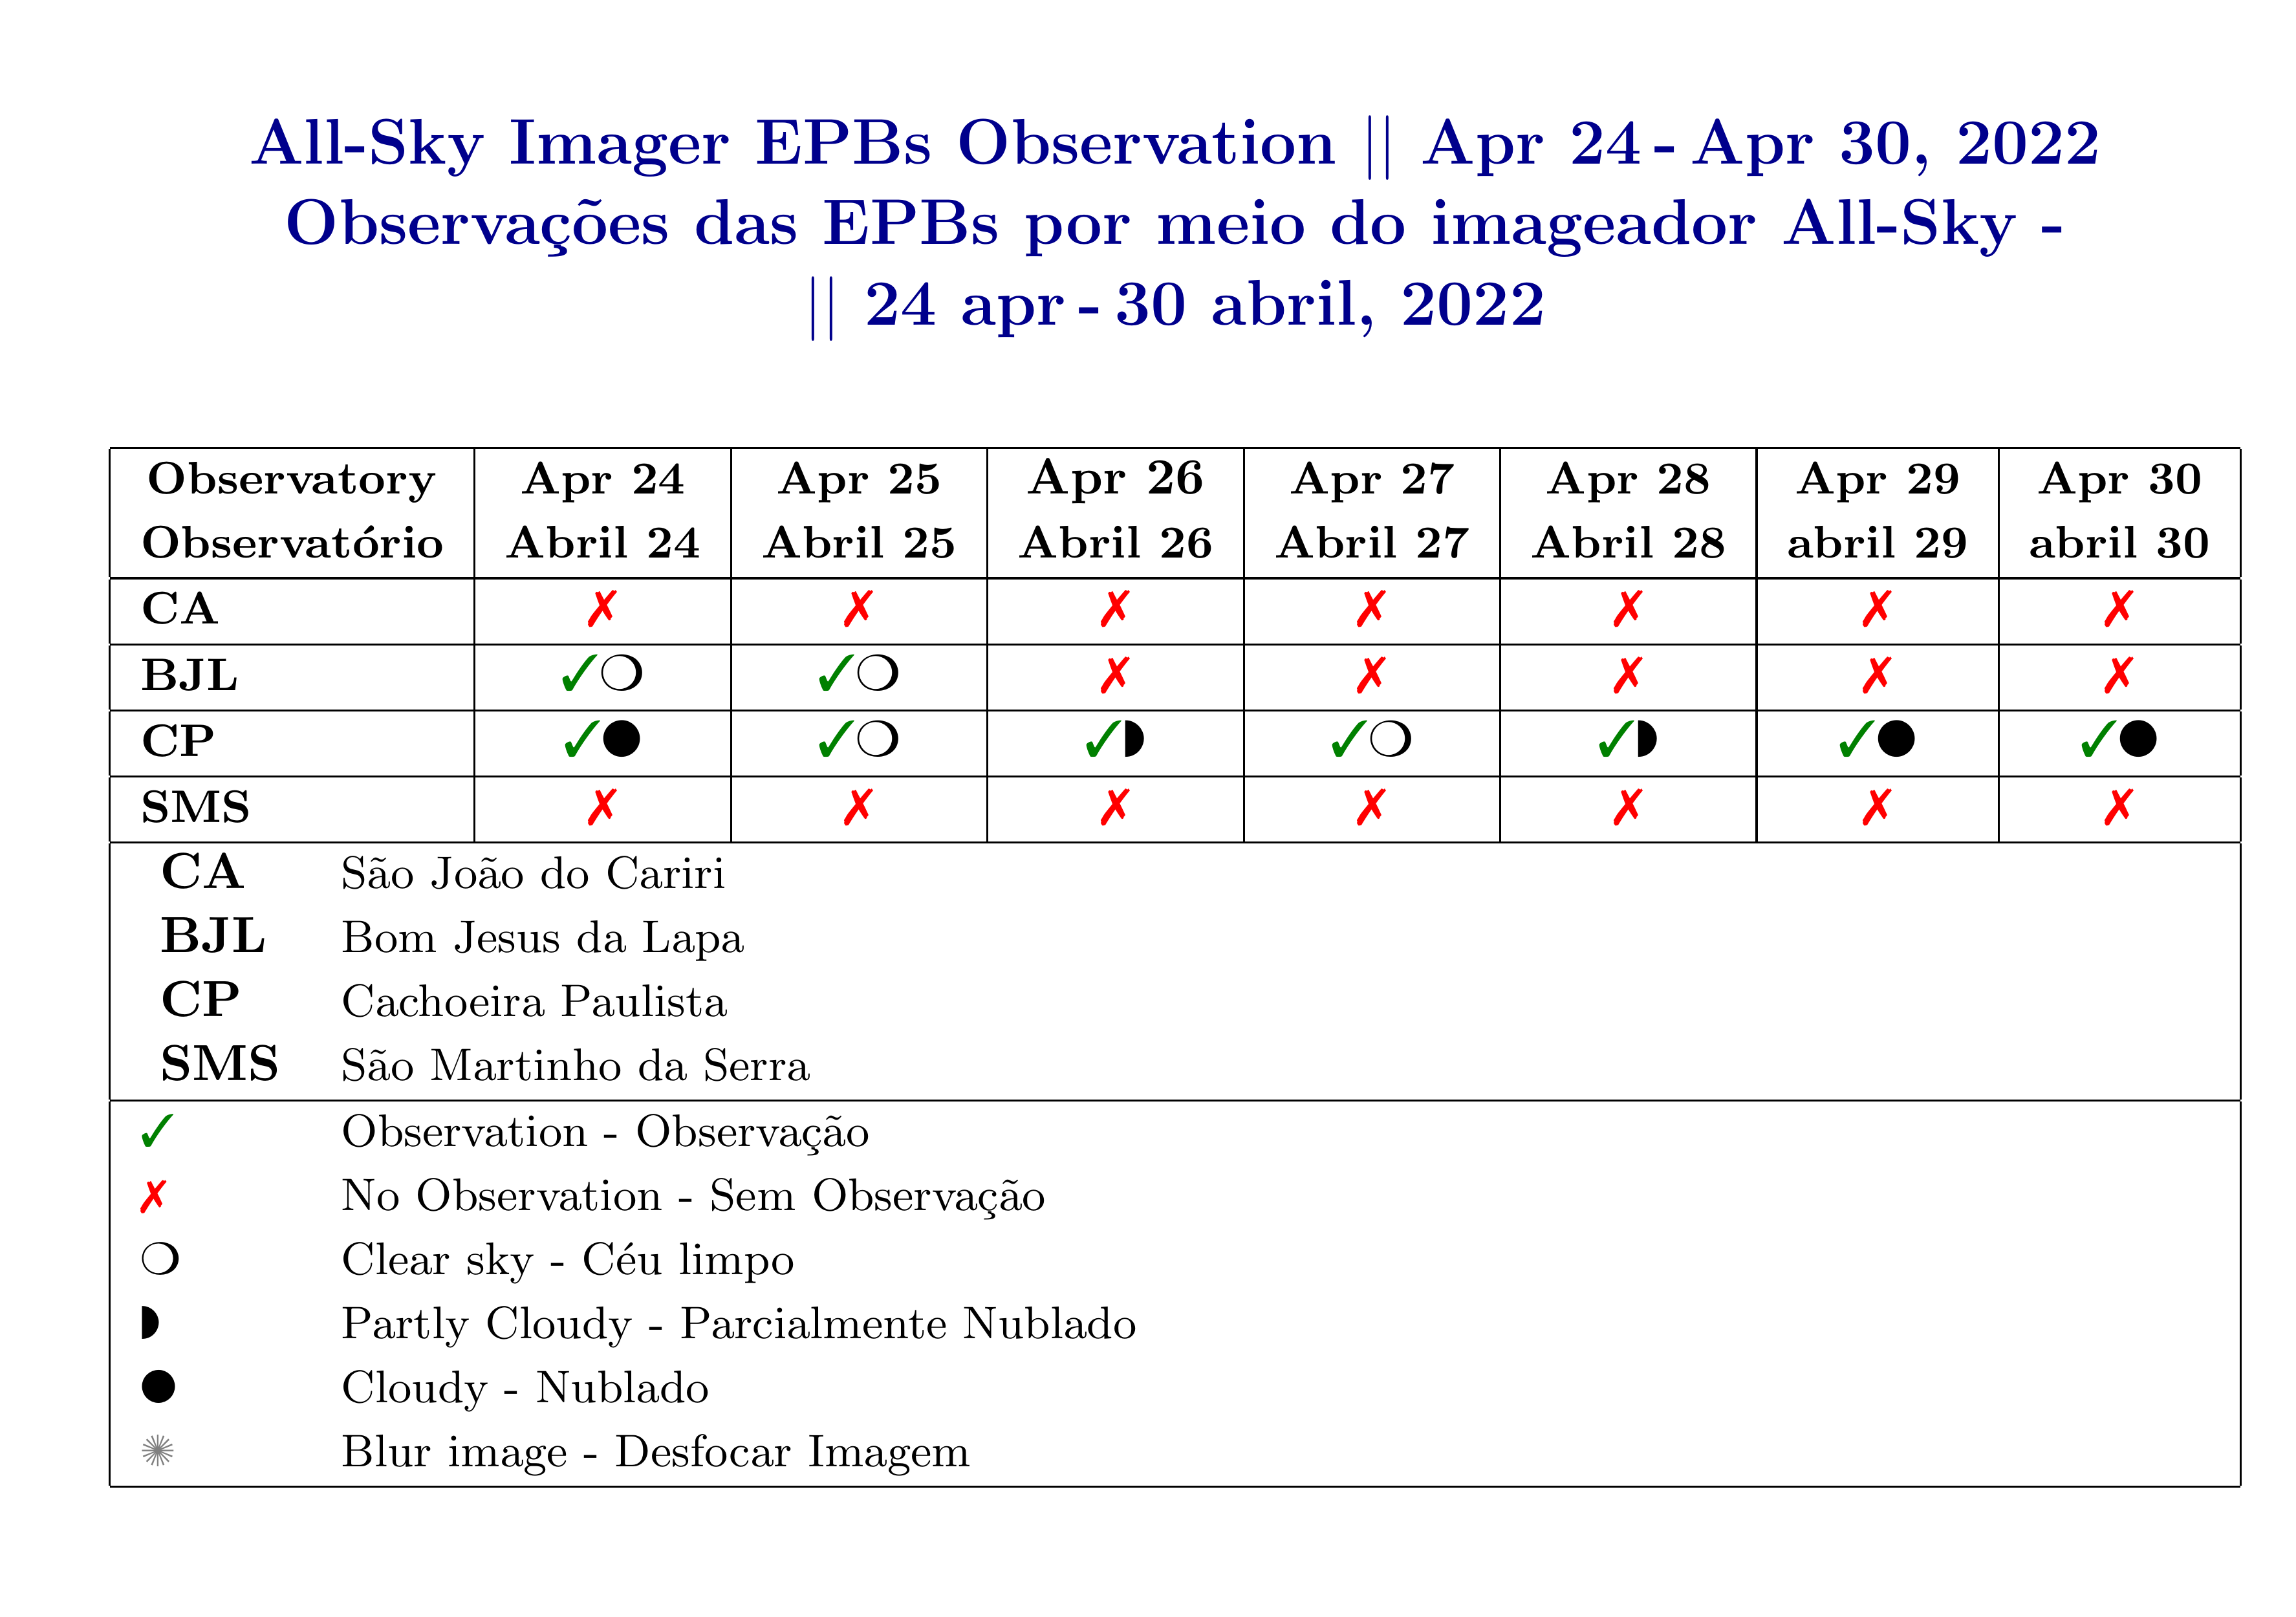
\includegraphics[width=14cm]{./figures//figureImager_0.png}

                        \end{figure}

                     \begin{itemize} 
 \item  At the Sao Joao do Cariri observatory, a small plasma bubble structure was observed on the night of May 3-4. Besides, on the night of May 06- 07, a traveling ionospheric disturbances was observed propagating to the northeast. 
\item  At the Bom de Jesus da Lapa observatory there was no observation due to technical problems. 
\item  At the Cachoeira Paulista no plasma bubbles were observed during the entire week even though there were observation. 
\item  Finally, at the observatory of Sao Martinho da Serra, no plasma bubble structures were observed during the entire week. 2 
\end{itemize} 
 TEC 
\begin{itemize} 
 \item  No plasma bubbles were observed during the entire period. As bubble sea- sonality is at the end, plasma bubbles have small spatial dimensions and they are difficult to observe on TEC maps.  3 
\end{itemize} 
 \section{ROTI} 
 \subsection{Responsible: Name} 
 
ROTI did not show significant variations related to ionospheric irregularities during the week. However, it is interesting to mention that some structures appear in the northern region of Brazil every day of the week. However, this region has low spatial coverage of GNSS receivers, and there are also the border's effects on the maps, causing an error propagation in this specific region.



\end{document}